% Options for packages loaded elsewhere
\PassOptionsToPackage{unicode}{hyperref}
\PassOptionsToPackage{hyphens}{url}
%
\documentclass[
  stu,floatsintext]{apa7}
\usepackage{amsmath,amssymb}
\usepackage{iftex}
\ifPDFTeX
  \usepackage[T1]{fontenc}
  \usepackage[utf8]{inputenc}
  \usepackage{textcomp} % provide euro and other symbols
\else % if luatex or xetex
  \usepackage{unicode-math} % this also loads fontspec
  \defaultfontfeatures{Scale=MatchLowercase}
  \defaultfontfeatures[\rmfamily]{Ligatures=TeX,Scale=1}
\fi
\usepackage{lmodern}
\ifPDFTeX\else
  % xetex/luatex font selection
\fi
% Use upquote if available, for straight quotes in verbatim environments
\IfFileExists{upquote.sty}{\usepackage{upquote}}{}
\IfFileExists{microtype.sty}{% use microtype if available
  \usepackage[]{microtype}
  \UseMicrotypeSet[protrusion]{basicmath} % disable protrusion for tt fonts
}{}
\makeatletter
\@ifundefined{KOMAClassName}{% if non-KOMA class
  \IfFileExists{parskip.sty}{%
    \usepackage{parskip}
  }{% else
    \setlength{\parindent}{0pt}
    \setlength{\parskip}{6pt plus 2pt minus 1pt}}
}{% if KOMA class
  \KOMAoptions{parskip=half}}
\makeatother
\usepackage{xcolor}
\usepackage{graphicx}
\makeatletter
\def\maxwidth{\ifdim\Gin@nat@width>\linewidth\linewidth\else\Gin@nat@width\fi}
\def\maxheight{\ifdim\Gin@nat@height>\textheight\textheight\else\Gin@nat@height\fi}
\makeatother
% Scale images if necessary, so that they will not overflow the page
% margins by default, and it is still possible to overwrite the defaults
% using explicit options in \includegraphics[width, height, ...]{}
\setkeys{Gin}{width=\maxwidth,height=\maxheight,keepaspectratio}
% Set default figure placement to htbp
\makeatletter
\def\fps@figure{htbp}
\makeatother
\setlength{\emergencystretch}{3em} % prevent overfull lines
\providecommand{\tightlist}{%
  \setlength{\itemsep}{0pt}\setlength{\parskip}{0pt}}
\setcounter{secnumdepth}{-\maxdimen} % remove section numbering
% Make \paragraph and \subparagraph free-standing
\ifx\paragraph\undefined\else
  \let\oldparagraph\paragraph
  \renewcommand{\paragraph}[1]{\oldparagraph{#1}\mbox{}}
\fi
\ifx\subparagraph\undefined\else
  \let\oldsubparagraph\subparagraph
  \renewcommand{\subparagraph}[1]{\oldsubparagraph{#1}\mbox{}}
\fi
% definitions for citeproc citations
\NewDocumentCommand\citeproctext{}{}
\NewDocumentCommand\citeproc{mm}{%
  \begingroup\def\citeproctext{#2}\cite{#1}\endgroup}
\makeatletter
 % allow citations to break across lines
 \let\@cite@ofmt\@firstofone
 % avoid brackets around text for \cite:
 \def\@biblabel#1{}
 \def\@cite#1#2{{#1\if@tempswa , #2\fi}}
\makeatother
\newlength{\cslhangindent}
\setlength{\cslhangindent}{1.5em}
\newlength{\csllabelwidth}
\setlength{\csllabelwidth}{3em}
\newenvironment{CSLReferences}[2] % #1 hanging-indent, #2 entry-spacing
 {\begin{list}{}{%
  \setlength{\itemindent}{0pt}
  \setlength{\leftmargin}{0pt}
  \setlength{\parsep}{0pt}
  % turn on hanging indent if param 1 is 1
  \ifodd #1
   \setlength{\leftmargin}{\cslhangindent}
   \setlength{\itemindent}{-1\cslhangindent}
  \fi
  % set entry spacing
  \setlength{\itemsep}{#2\baselineskip}}}
 {\end{list}}
\usepackage{calc}
\newcommand{\CSLBlock}[1]{\hfill\break\parbox[t]{\linewidth}{\strut\ignorespaces#1\strut}}
\newcommand{\CSLLeftMargin}[1]{\parbox[t]{\csllabelwidth}{\strut#1\strut}}
\newcommand{\CSLRightInline}[1]{\parbox[t]{\linewidth - \csllabelwidth}{\strut#1\strut}}
\newcommand{\CSLIndent}[1]{\hspace{\cslhangindent}#1}
\ifLuaTeX
\usepackage[bidi=basic]{babel}
\else
\usepackage[bidi=default]{babel}
\fi
\babelprovide[main,import]{british}
% get rid of language-specific shorthands (see #6817):
\let\LanguageShortHands\languageshorthands
\def\languageshorthands#1{}
% Manuscript styling
\usepackage{upgreek}
\captionsetup{font=singlespacing,justification=justified}

% Table formatting
\usepackage{longtable}
\usepackage{lscape}
% \usepackage[counterclockwise]{rotating}   % Landscape page setup for large tables
\usepackage{multirow}		% Table styling
\usepackage{tabularx}		% Control Column width
\usepackage[flushleft]{threeparttable}	% Allows for three part tables with a specified notes section
\usepackage{threeparttablex}            % Lets threeparttable work with longtable

% Create new environments so endfloat can handle them
% \newenvironment{ltable}
%   {\begin{landscape}\centering\begin{threeparttable}}
%   {\end{threeparttable}\end{landscape}}
\newenvironment{lltable}{\begin{landscape}\centering\begin{ThreePartTable}}{\end{ThreePartTable}\end{landscape}}

% Enables adjusting longtable caption width to table width
% Solution found at http://golatex.de/longtable-mit-caption-so-breit-wie-die-tabelle-t15767.html
\makeatletter
\newcommand\LastLTentrywidth{1em}
\newlength\longtablewidth
\setlength{\longtablewidth}{1in}
\newcommand{\getlongtablewidth}{\begingroup \ifcsname LT@\roman{LT@tables}\endcsname \global\longtablewidth=0pt \renewcommand{\LT@entry}[2]{\global\advance\longtablewidth by ##2\relax\gdef\LastLTentrywidth{##2}}\@nameuse{LT@\roman{LT@tables}} \fi \endgroup}

% \setlength{\parindent}{0.5in}
% \setlength{\parskip}{0pt plus 0pt minus 0pt}

% Overwrite redefinition of paragraph and subparagraph by the default LaTeX template
% See https://github.com/crsh/papaja/issues/292
\makeatletter
\renewcommand{\paragraph}{\@startsection{paragraph}{4}{\parindent}%
  {0\baselineskip \@plus 0.2ex \@minus 0.2ex}%
  {-1em}%
  {\normalfont\normalsize\bfseries\itshape\typesectitle}}

\renewcommand{\subparagraph}[1]{\@startsection{subparagraph}{5}{1em}%
  {0\baselineskip \@plus 0.2ex \@minus 0.2ex}%
  {-\z@\relax}%
  {\normalfont\normalsize\itshape\hspace{\parindent}{#1}\textit{\addperi}}{\relax}}
\makeatother

\makeatletter
\usepackage{etoolbox}
\patchcmd{\maketitle}
  {\section{\normalfont\normalsize\abstractname}}
  {\section*{\normalfont\normalsize\abstractname}}
  {}{\typeout{Failed to patch abstract.}}
\patchcmd{\maketitle}
  {\section{\protect\normalfont{\@title}}}
  {\section*{\protect\normalfont{\@title}}}
  {}{\typeout{Failed to patch title.}}
\makeatother

\usepackage{xpatch}
\makeatletter
\xapptocmd\appendix
  {\xapptocmd\section
    {\addcontentsline{toc}{section}{\appendixname\ifoneappendix\else~\theappendix\fi\\: #1}}
    {}{\InnerPatchFailed}%
  }
{}{\PatchFailed}
\keywords{keywords\newline\indent Word count: X}
\usepackage{csquotes}
\usepackage[titles]{tocloft}
\cftpagenumbersoff{figure}
\renewcommand{\cftfigpresnum}{\itshape\figurename\enspace}
\renewcommand{\cftfigaftersnum}{.\space}
\setlength{\cftfigindent}{0pt}
\setlength{\cftafterloftitleskip}{0pt}
\settowidth{\cftfignumwidth}{Figure 10.\qquad}
\cftpagenumbersoff{table}
\renewcommand{\cfttabpresnum}{\itshape\tablename\enspace}
\renewcommand{\cfttabaftersnum}{.\space}
\setlength{\cfttabindent}{0pt}
\setlength{\cftafterloftitleskip}{0pt}
\settowidth{\cfttabnumwidth}{Table 10.\qquad}
\makeatletter
\renewcommand{\paragraph}{\@startsection{paragraph}{4}{\parindent}%
  {0\baselineskip \@plus 0.2ex \@minus 0.2ex}%
  {-1em}%
  {\normalfont\normalsize\bfseries\typesectitle}}

\renewcommand{\subparagraph}[1]{\@startsection{subparagraph}{5}{1em}%
  {0\baselineskip \@plus 0.2ex \@minus 0.2ex}%
  {-\z@\relax}%
  {\normalfont\normalsize\bfseries\itshape\hspace{\parindent}{#1}\textit{\addperi}}{\relax}}
\makeatother
\setlength{\cslhangindent}{0.5in}
\usepackage{fancyhdr} 
\pagestyle{fancy}   
\fancyhf{} 
\fancyhead[R]{\thepage} 
\renewcommand{\headrulewidth}{0pt}
\thispagestyle{fancy}
\duedate{07.08.2023}
\course{Modul 6b: Empirisch-Experimentelles Praktikum}
\professor{Dr. }

\ifLuaTeX
  \usepackage{selnolig}  % disable illegal ligatures
\fi
\usepackage{bookmark}
\IfFileExists{xurl.sty}{\usepackage{xurl}}{} % add URL line breaks if available
\urlstyle{same}
\hypersetup{
  pdftitle={The title},
  pdfauthor={First Author1 \& Ernst-August Doelle1,2},
  pdflang={en-GB},
  pdfkeywords={keywords},
  hidelinks,
  pdfcreator={LaTeX via pandoc}}

\title{The title}
\author{First Author\textsuperscript{1} \& Ernst-August Doelle\textsuperscript{1,2}}
\date{}


\shorttitle{Title}

\authornote{

Add complete departmental affiliations for each author here. Each new line herein must be indented, like this line.

Enter author note here.

The authors made the following contributions. First Author: Conceptualization, Writing - Original Draft Preparation, Writing - Review \& Editing; Ernst-August Doelle: Writing - Review \& Editing, Supervision.

Correspondence concerning this article should be addressed to First Author, Postal address. E-mail: \href{mailto:my@email.com}{\nolinkurl{my@email.com}}

}

\affiliation{\vspace{0.5cm}\textsuperscript{1} Wilhelm-Wundt-University\\\textsuperscript{2} Konstanz Business School}

\note{\clearpage}

\abstract{%
One or two sentences providing a \textbf{basic introduction} to the field, comprehensible to a scientist in any discipline.
Two to three sentences of \textbf{more detailed background}, comprehensible to scientists in related disciplines.
One sentence clearly stating the \textbf{general problem} being addressed by this particular study.
One sentence summarizing the main result (with the words ``\textbf{here we show}'' or their equivalent).
Two or three sentences explaining what the \textbf{main result} reveals in direct comparison to what was thought to be the case previously, or how the main result adds to previous knowledge.
One or two sentences to put the results into a more \textbf{general context}.
Two or three sentences to provide a \textbf{broader perspective}, readily comprehensible to a scientist in any discipline.
}



\begin{document}
\maketitle

\section{Methods}\label{methods}

\subsection{Preregistration and version control}\label{preregistration-and-version-control}

The hypotheses, the inclusion/exclusion criteria, used databases, search queries and the basic theoretical foundation of this systematic literature review are preregistered and can be found on Moodle or in the GitHub repository.\\
As suggested by Lakens (2022) (Chapter 14), the present systemic literature used a GitHub repository to store all data and files. The repository is available at: \url{https://github.com/julianrottenberg/Stereotype_Threat_im_akademischen_Kontext}\\
This approach allows for more transparency and reproducibility as well as accountability.

\subsection{Artificial Intelligence (AI)}\label{artificial-intelligence-ai}

It should be acknowledged that artificial intelligence has been used as an aid in this review - namely, Anthropic's Claude AI 3.5 Sonnet (Anthropic, 2024) and GitHub's Copilot (GitHub \& OpenAi, 2024), the latter was directly integrated into RStudio Server (Posit team, 2024). The chats that directly influenced this review are all available on the GitHub repository.
For Github Copilot the autocomplete-style suggestions were used.\\
Claude AI 3.5 Sonnet was used to generate descriptions of the papers used in this review - based on a template, further, follow up questions were asked to clear up uncertainties.
The process here was as follows: First the template was manually filled out by a human, after this process was completed for every paper, a second template was created, the contents of which were filled out by AI and then, later, used in conjunction with the manually created templates. When the different templates differed from one another the primary source (i.e.~the paper the template was based on) was checked again. Both, the human-generated as well as the AI-generated templates can be found on the GitHub repository - the AI generated summaries have been marked as such, beginning with ``Claude\_Ai\_'' in their file name.\\
To clarify, AI was not used to generate any of the text in this review, it was used as a tool to gather a better understanding and overview of the papers involved. The process of having a human and AI created summary of each paper was chosen to gather an extra layer of security regarding the contents of each paper as well as to counteract possible oversights.

\subsection{Databases, search queries and inclusion/exclusion criteria}\label{databases-search-queries-and-inclusionexclusion-criteria}

The databases used were Web of Science, Google Scholar, PSYNDEX, ResearchRabbit and EBSCOhost Within EBSCOhost, the databases APA PsycArticles, APA PsycInfo, Psychology and Behavioral Sciences Collection, PSYNDEX Literature with PSYNDEX Tests, Education Source Ultimate, and Academic Search Ultimate were searched.\\
Furthermore, the snowball method was utilised to find additional papers - however, this approach did not deliver any additional papers, the same applies to ResearchRabbit.\\
The permalinks to each search used can also be found within the GitHub repository.\\
Within Web of Science the included document types were ``Article'', ``Other'', or ``Clinical Trail''; the excluded document types were ``Book'', ``Meeting'', ``Editorial Material'', or ``Review Article''.
Furthermore, the database ``Preprint Citation Index'' was excluded.\\
In EBSCOhost, ``Apply equivalent subjects'' was applied as an Expander, while ``Peer Reviewed'', ``Document Type*'', and ``Publication Type*'' were used as Limiters.\\
In Google Scholar, the following was added at the end of the search query: ``AND''empirical study'' AND ``peer-reviewed'' -books -meta-analysis)``.\\
These extra filters were applied in accordance with the inclusion and exclusion criteria outlined in the preregistration. No other changes were made to the search queries. An overview of the search queries can be found in Table \ref{tab:query_table}.

\begin{table}[tbp]

\begin{center}
\begin{threeparttable}

\caption{\label{tab:query_table}Search queries used for the systematic literature review.}

\begin{tabular}{m{4cm}m{12cm}}
\toprule
Hypothesis & \multicolumn{1}{c}{Search Query}\\
\midrule
H1 & ("stereotype threat") AND 
(neural OR neuroimaging OR "functional magnetic resonance imaging" OR fMRI OR electroencephalo* OR EEG OR ERP OR "brain activation" OR amygdala OR "prefrontal cortex" OR "default mode network" OR "salience network") AND
(academ* OR education* OR stud* OR learn* OR perform* OR school OR university OR college)\\
H2 & ("stereotype threat") AND 
("cognitive control" OR "executive function" OR "executive function network" OR "cognitive control network" OR "brain activation" OR "brain activation patterns" OR "cognitive tasks" OR "executive tasks" OR "cognitive assessment" OR "executive assessment") AND 
(academ* OR education* OR stud* OR learn* OR perform* OR school OR university OR college)\\
H3 & ("stereotype threat") AND 
("working memory*" OR "processing speed" OR accuracy) AND 
(academ* OR education* OR stud* OR learn* OR perform* OR school OR university OR college)\\
\bottomrule
\addlinespace
\end{tabular}

\begin{tablenotes}[para]
\normalsize{\textit{Note.} The search queries were used in the databases Web of Science, Google Scholar, PSYNDEX, ResearchRabbit, and EBSCOhost. The permalinks to each search used can be found within the GitHub repository.}
\end{tablenotes}

\end{threeparttable}
\end{center}

\end{table}

The inclusion and exclusion criteria specified in the preregistration were applied to each paper.
The criteria ``Stereotype Threat'', which required studies to ``explicitly examine, manipulate, or measure stereotype threat as a key study variable or factor'' was enforced on a lot of papers and resulted in their exclusion - even when they were otherwise relevant (more on this in the discussion section), same applies to the ``Outcomes'' criteria, which required studies to report ``at least one of the following: 1. Neural activation patterns/brain imaging data; 2. Cognitive processes (e.g., working memory, cognitive control/executive functions)'' also resulted in the exclusion of papers which indirectly measured these outcomes but/or did not specifically focus on ``working memory'' for example - as an example: a paper might have used a test that is known to measure working memory but did not mention ``working memory'' within its abstract, methods or results section, so it was excluded.

\subsection{Screening and paper details}\label{screening-and-paper-details}

The screening process was done using the software Rayyan (Ouzzani et al., 2016). All results were imported onto the platform.
The total amount of papers found was 599 (\(N=599\), \(n_{\text{EBSCOhost}} = 105\), \(n_{\text{Google Scholar}} = 48\), \(n_{\text{PSYNDEX}} = 5\), \(n_{\text{ResearchRabbit}} = 4\), \(n_{\text{Web of Science}} = 437\)). Out of these 83 were duplicates (88 were automatically detected by Rayyan, however, 5 were false positives), leaving 516 papers to be screened. During the first screening another 440 papers were excluded.
Papers which were excluded did not fit the inclusion criteria, most prominently, they either did not focus on stereotype threat, had the wrong population (e.g., older adults), did not fit the publication type requirements, or did not measure the outcomes of interest - this was assessed using the title, keywords, and abstract. If neither the title, nor the keywords or abstract mentioned enough information to make a decision, the paper was marked as `maybe.
An example for hypothesis 3 would be, a paper measured working memory but just referred to ``the participants'' in the abstract, without clarifying that they fit the definition of the academic context. After this first screening, 76 papers remained for the second screening.
This second screening was done by looking into the full-text of each paper, here another 44 papers were excluded for the following reasons: wrong focus (\(n = 29\)), wrong population (\(n = 7\)), wrong study design (\(n = 5\)), wrong publication type (\(n = 2\)) - an overview of this can be found in the PRISMA flowchart (Haddaway et al., 2022) in Figure \ref{fig:prisma}.
In the end, 32 papers were included in this review, \(n = 8\) for hypothesis 1, \(n = 9\) for hypothesis 2, and \(n = 19\) for hypothesis 3 - some were used for multiple hypotheses. Out of the 516 papers, 319 were excluded for 'wrong focus', 56 for `wrong population', 14 for `wrong study design', 12 for wrong publication type, 2 for `foreign language', and 1 for `wrong study duration' (some papers were excluded for multiple reasons). A full list of all papers found and excluded can be found in the GitHub repository.\\
A template was created to summarise each paper, with two versions completed: one by the author and one by Claude AI.
The template was a mixture of the following checklists: CASP systematic review checklist (Critical Appraisal Skills Programme, 2018), Review guidelines for extracting data and quality assessing primary studies in educational research (EPPI-Centre, 2003), Critical appraisal checklist for a systematic review (University of Glasgow, n.d.), and the Newcastle-Ottawa scale (NOS) for assessing the quality of nonrandomised studies in meta-analyses (Wells et al., 2014), which are used to describe studies and assess their quality.
Redundant and irrelevant items were eliminated, and the remaining questions were consolidated into a single template.
This approach provided a comprehensive overview of the final papers.
Based on these summaries, the papers were analysed and the results are presented in the following sections.

\begin{figure}
\centering
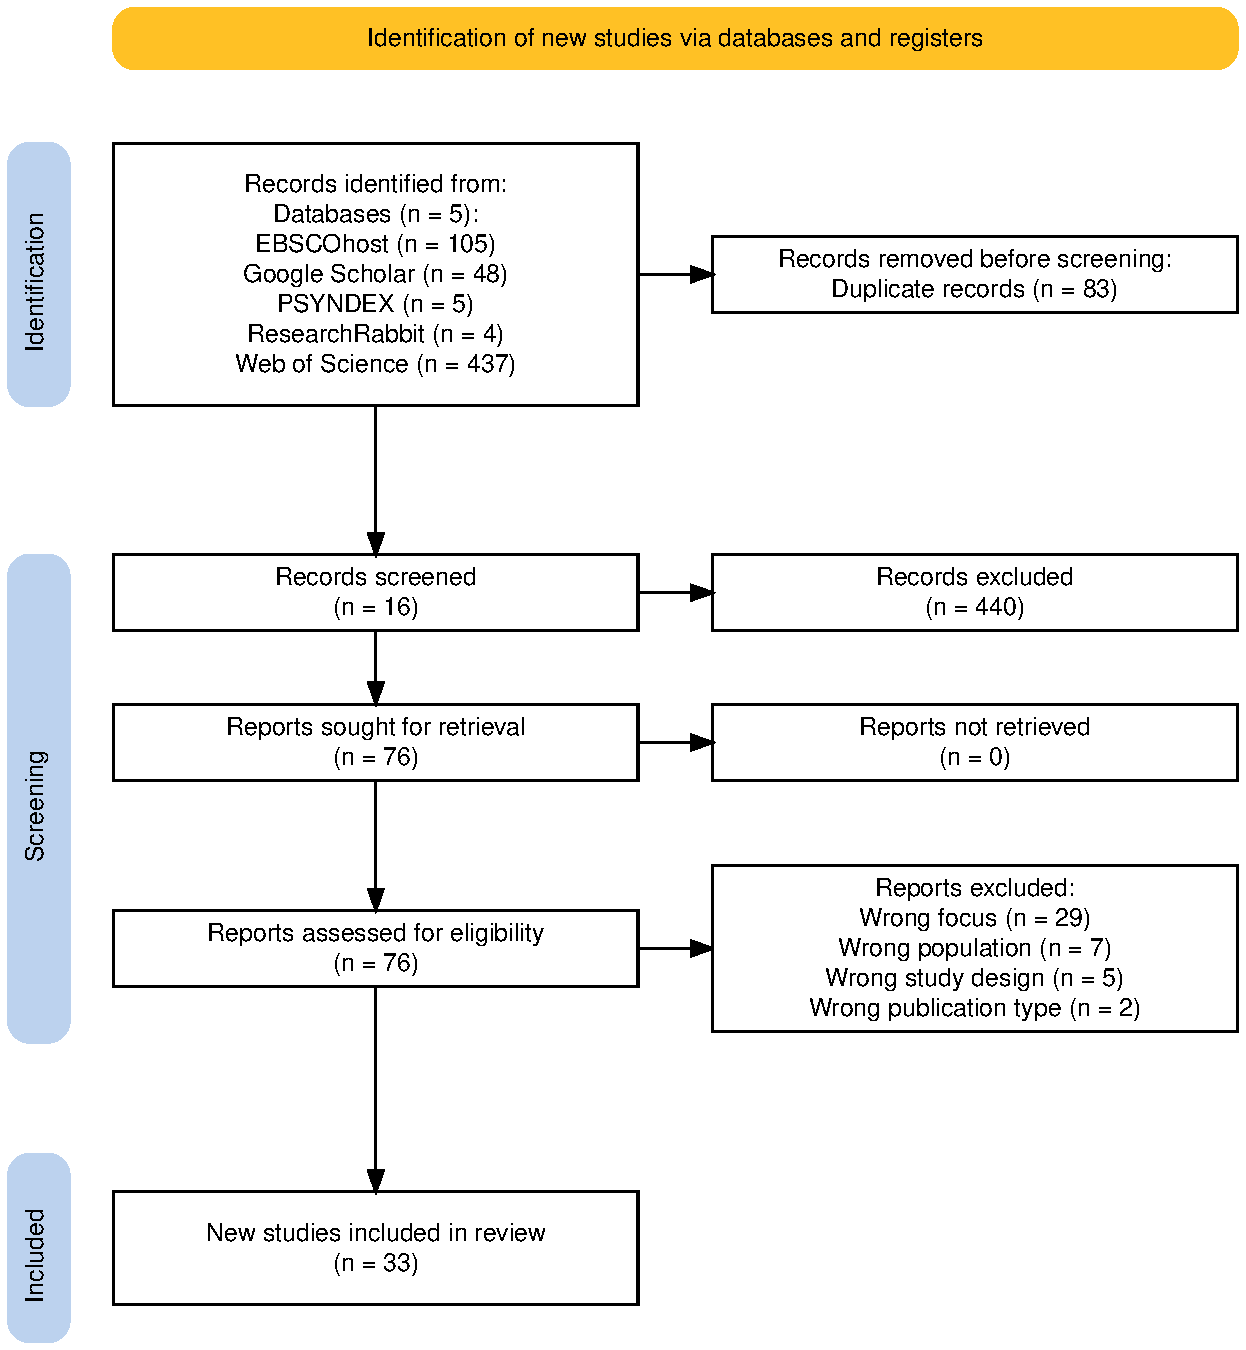
\includegraphics{files/prisma.pdf}
\caption{\label{fig:prisma}PRISMA flowchart of the screening process.}
\end{figure}

\subsection{RStudio and R packages}\label{rstudio-and-r-packages}

The following R packages were used to create this review: R (Version 4.4.1; R Core Team, 2024) and the R-packages \emph{citr} (Version 0.3.2; Aust, 2019), \emph{kableExtra} (Version 1.4.0; Zhu, 2024), \emph{papaja} (Version 0.1.2.9000; Aust \& Barth, 2023), \emph{RefManageR} (Version 1.4.0; McLean, 2017), \emph{rmarkdown} (Version 2.27; Xie et al., 2018, 2020), and \emph{tinylabels} (Version 0.2.4; Barth, 2023).

\section{Results}\label{results}

\subsection{Results Hypothesis 1: Stereotype threat induces variations in neutral activation across different brain areas and networks, potentially influencing academic performance. These may include the amygdala, the prefrontal cortex, the default mode network, and the salience network.}\label{results-hypothesis-1-stereotype-threat-induces-variations-in-neutral-activation-across-different-brain-areas-and-networks-potentially-influencing-academic-performance.-these-may-include-the-amygdala-the-prefrontal-cortex-the-default-mode-network-and-the-salience-network.}

\subsubsection{Beilock et al. (2007)}\label{beilockstereotypethreatworking2007}

In their paper, Beilock et al. (2007) focussed on stereotypes effects on working memory, specifically, which parts of working memory are affected by stereotype threat and when these effects linger on and influence performance on unrelated tasks.
To investigate this, they focussed on maths stereotype threat, their population consisted of female college students in the United States.
Their paper describes five experiments, all of which used a cross-sectional design.
Experiment 1, 3 (both A and B), and Experiment 5, consisted of two groups each, with `stereotype threat' vs.~`no stereotype threat', `horizontal vs.~vertical modular arithmetic (MA) conditions', and `spatial two-back vs.~verbal two-back task', respectively, each with random allocation.
Experiment 2 and 4 consisted of one group each.
Since neither Experiment 2 nor 3B were relevant to the hypotheses for this review, they will not be discussed further.
Across all experiments, participants were female undergraduate students.

\paragraph{Modular Arithmetic (MA) task}\label{modular-arithmetic-ma-task}

The MA task was used to measure maths performance.
Participants were asked to judge the validity of equations, like \(60 = 19 mod(4)\), which would result in \(false\).
These equations were either displayed vertically or horizontally and consisted of varying difficulty, thus differed in working memory demand.
Using this type of task allowed the researchers to measure the effect stereotype threat had on working memory.

\paragraph{Two-back task}\label{two-back-task}

Participants were given a stimuli and had to decide whether or not the given stimuli matched the one presented two trials before.
The stimuli in use were a cluster of identical letters (e.g., \emph{cs}, \emph{ns}) and one of six different spatial locations in an ellipse.
The two-back task was split into a verbal (letters) or spatial (locations) version, participants were randomly assigned to one of these versions.

\paragraph{Experiment 1}\label{experiment-1}

\(N = 31\) women, of equal self-reported maths skill participated in this experiment, \(n_{\text{stereotype threat}} = 14\), \(n_{\text{no stereotype threat}} = 17\).
Firstly, participants were introduced to the MA task, and were then asked to solve 12 practice problems, these differed in demand but only consisted of horizontal problems.
Afterwards, 24 problems were performed by each participant over two blocks, with the first one serving as a baseline and the second as the posttest.
Stereotype threat manipulation was performed in between these blocks via text on a computer screen.
An adaptation of the stereotype threat manipulation used by Aronson et al. (1999) was used by displaying the text on a computer screen.
Maths accuracy and reaction time were measured as dependent variables, while Group (stereotype threat vs.~control), Problem working memory demand (low vs.~high), and Block (baseline vs.~posttest) functioned as independent variables.\\
Within the stereotype threat condition \(\text{Group } \times \text{ Block } \times \text{ Problem Demand }\), \emph{F}(1,29) = 11.18, \emph{p} \textless{} .010, \(\eta^{2}_{p}\) = 0.28, resulted in a significant interaction effect for accuracy.
Further, \(\text{Group } \times \text{ Block } \times \text{ Problem Demand }\), on reaction time, showed main effect of block, and problem demand; \emph{F}(1,29) = 8.33, \emph{p} \textless{} .010, \(\eta^{2}_{p}\) = 0.22, and \emph{F}(1,29) = 754.5, \emph{p} \textless{} .010, \(\eta^{2}_{p}\) = 0.96, respectively.
Thus, individuals were able to increase their speed over time and the more demanding a problem was, the longer it took to solve it.
A comparison of the accuracy between the baseline and posttest within the stereotype threat condition showed no difference in terms of accuracy for low-demand problems, while, for high-demand problems, a significant decrease in accuracy between the posttest (\emph{M} = 79.3\%, \emph{SE} = 4.6\%) and baseline (\emph{M} = 89.1\%, \emph{SE} = 3.8\%) was found; CI {[}81.00\% - 97.00\%{]}; \emph{d} = 0.61.\\
Beilock et al. (2007) conclude that only high- but not low-demand problems affect working memory under stereotype threat.

\paragraph{Experiment 3A}\label{experiment-3a}

Here, a sample of thirty-three (\(N = 33\)) women performed, both, vertical and horizontal MA tasks.
Similar to Experiment 1 they were introduced to the subject with a practice block, followed by a baseline block and a posttest block.
This time, all participants received the stereotype threat manipulation in between the last two blocks but were randomly assigned to either the vertical or horizontal problem condition.
Afterwards, they were given questionnaires to assess their thought during the stereotype threat manipulation, their perceived importance of task performance, and their state anxiety following stereotype threat.
The independent variables consisted of Block (baseline vs.~stereotype threat), Problem working memory demand (low vs.~high), and Problem orientation (horiztonal vs.~vertical), while the dependent variables were maths problem accuracy, reaction times, and self-reported thoughts/worries.
Neither the perceived importance of performing well (vertical: \emph{M} = 4.67, \emph{SE} = 0.35; horizontal: \emph{M} = 5.27, \emph{SE} = 0.37) nor state anxiety differed between the groups (vertical: \emph{M} = 33.22, \emph{SE} = 1.6; horizontal: \emph{M} = 37.00, \emph{SE} = 2.7), \emph{F}(1,31) = 1.53, \emph{p} = .220.
Thoughts/worries were split into four categories, most common were thoughts about the performance monitoring (34.9\%), followed by thoughts related about the processes involved in solving the problems (32.4\%), unrelated thoughts made up 18.3\% and, lastly, 14.5\% of the thoughts related to the stereotype threat manipulation.
Again, no significant difference between the groups was found (Categories 1, 3, and 4: \emph{F} \textless{} 1; Category 2: \emph{F}(1,31) = 2.17, \emph{p} = .150.)\\
For the MA problems, a three-way interaction between the independent variables was found, \emph{F}(1,31) = 4.12, \emph{p} = .050, \(\eta^{2}_{p}\) = 0.12.\\
Similar to Experiment 1, a significant \(\text{Block } \times \text{Problem Demand }\) interaction was found but only for horizontal problems, \emph{F}(1,14) = 7.70, \emph{p} \textless{} .020, \(\eta^{2}_{p}\) = 0.36.
Accuracy suffered significantly from the baseline (\emph{M} = 91.7\%, \emph{SE} = 3.6\%) to the stereotype threat (\emph{M} = 81.2\%, SE = 4.6\%) block; CI {[}84.00\% - 99.30\%{]}; \emph{d} = 0.64.
The three-way ANOVA for, RTs revealed that high-demand problems were slower, compared to low-demand problems; vertical: \emph{F}(1,17) = 306.32, \emph{p} \textless{} .010, \(\eta^{2}_{p}\) = 0.95; horizontal: \emph{F}(1,14) = 11.04, \emph{p} \textless{} .010, \(\eta^{2}_{p}\) = 0.44.
This effect was not significant for horizontal problems and revealed a main effect for vertical problems.\\
It is concluded that low-demand problems do not suffer under stereotype threat, however, the working memory is impaired for high-demand problems resulting in a decrease in accuracy (only for horizontal problems) and an increase in reaction time.

\paragraph{Experiment 4}\label{experiment-4}

All thirty (\(N = 30\)) women were tasked to solve horizontal and vertical MA under stereotype threat.
Procedure was similar to Experiment 3A, albeit, with a bigger practice block, and the repetition of some problems.
The independent variables consisted of Block (baseline vs.~stereotype threat), Problem Repetition (no repeat vs.~multiple repeat), and Problem Working Memory demand (low vs.~high), while the dependent variables did not differ from Experiment 1.
The significant \(\text{Block } \times \text{ Problem Repetition } \times\) \(\text{ Problem Working Memory demand }\) interaction, \emph{F}(1, 29) = 6.13, \emph{p} \textless{} .020, \(\eta^{2}_{p}\) = 0.17, was further analysed by differentiating between multi- and no=repeat problems.\\
For the multi-repeat problems no significant interaction was to be found (\emph{F} \textless{} 1), meanwhile a significant effect was found for the no-repeat problems, \emph{F}(1,29) = 11.11, \emph{p} \textless{} 0.01, \(\eta^{2}_{p}\) = 0.28.
While the accuracy, again, significantly decreased from the baseline (\emph{M} = 65.00\%, \emph{SE} = 3.9\%) to the stereotype threat block (\emph{M} = 65.00\%, \emph{SE} = 5.9\%; CI {[}52.80\% - 77.20\%{]}; \emph{d} = 0.70) in high-demand problems, within the no-repeat condition, no significant effect was found for the low-demand problems (baseline: \emph{M} = 95.00\%, \emph{SE} = 1.50\%, stereotype threat: \emph{M} = 94.80\%, \emph{SE} = 2.80\%).
For the RTs, problem demand, \emph{F}(1,26) = 144.14, \emph{p} \textless{} .010, \(\eta^{2}_{p}\) = 0.85, influenced the RTs more than problem repetition,\emph{F}(1,26) = 139.94, \emph{p} \textless{} .010, \(\eta^{2}_{p}\) = 0.84, both showing main effects.\\
Based on these results, the authors conclude that practised, horizontal problems do not rely on working memory heavily, evidenced by them not being affected by stereotype threat.
The opposite is true for no-repeat problems, which did suffer under stereotype threat, given that they were of high verbal working memory demand.

\paragraph{Experiment 5}\label{experiment-5}

The last experiment was preceded by a pilot test to establish whether the two-back tasks were of equal difficulty.
This pilot test was done with \(N = 27\) women, without any stereotype threat manipulation, the procedure is similar to the main experiment, thus will not be discussed further.\\
The main experiment consisted of thirty-three (\(N = 33\)) women.
Upon arrival participants completed a two-back practise task, after changing computers, they practised the MA task.
Afterwards, the stereotype threat manipulation was performed, followed by twenty high-demand horizontal problems.
In the next step, participants went back to the first computer to complete 100 trails of the same version of the two-back task that was practised before.\\
Condition (stereotype threat vs.~control; control being the pilot test) and Two-back task type (verbal vs.~spatial) functioned as independent variables, while the dependent variables were accuracy and reaction time, each for, both, the maths problem and the two-back task.\\
Comparing the MA results with the previous experiments results for the same type of task (horizontal, high-demand), showed that the stereotype threat significantly inhibited performance (\emph{M} = 82.20\%, \emph{SE} = 2.00\%), while the same cannot be said for the no-threat conditions (\emph{M} = 91.50\%, \emph{SE} = 1.50\%).\\
For the two-back task, RTs between spatial (\emph{M} = 895 ms, \emph{SE} = 49 ms) and verbal (\emph{M} = 1087 ms, \emph{SE} = 59 ms) task differed significantly, \emph{F}(1,31) = 6.133, \emph{p} \textless{} .020, \(\eta^{2}_{p}\) = 0.17 while the difference in accuracy did not reach significance (verbal: \emph{M} = 87.30\%, \emph{SE} = 1.70\%; spatial: \emph{M} = 89.00\%, \emph{SE} = 1.50\%, \emph{F} \textless{} 1).
Comparing the performance of the stereotype threat condition with the control (pilot test), showed an interaction between \(\text{Task } \times \text{ Experiment }\) for RT, \emph{F}(1,56) = 4.38, \emph{p} \textless{} .050, \(\eta^{2}_{p}\) = 0.07.
Without stereotype threat, no significant differences in performance between thee verbal and spatial two-back tasks were found, however, under stereotype threat the verbal task was significantly slower than the spatial task.\\
Contrary to the previous Experiments, Experiment 5 additionally aimed to investigate whether stereotype threat has a spill over effect on unrelated tasks.
Since these results are not relevant to the hypotheses of this review, they will not be discussed in detail.
Using multiple regression analyses the authors found that the stereotype threat did indeed spill over to the two-back task, however, only for the verbal task.\\
According to the authors, the results of the different Experiments in this paper, show stereotype threats effect on working memory, they mention that ``especially the phonological aspects'' are affected.
Stereotype threat's effect onto task-related worries as well as thoughts serve as further indications for this conclusion.
Further, it is concluded that stereotype threat likely affects multiple aspects of working memory.
A combination of phonological loop and central executive functioning is suggested to be affected by stereotype threat.\\
H1 is partially confirmed by this paper, central executive functioning is assumed to involve the prefrontal cortex, however, this is not the only area affected.
The phonological loop is associated with BA4, BA49, and (approximately) BA44 and BA 45.

\subsubsection{Dunst et al. (2013)}\label{dunstsexdifferencesneural2013}

In a \(2 \text{ (sex: male vs. female) } \times 2 \text{ (stereotype exposure: stereotype threat vs. no stereotype threat) }\) cross-sectional between-subjects design, a mixed-sex sample of secondary school students in Austria, was used to investigate the effects of stereotype threat on neural efficiency as well as sex differences in visuo-spatial task performance.
The dependent variables consisted of task performance (accuracy and reaction time), brain activation (task-related-power changes), and neural efficiency (correlation between figural intelligence and brain activation); sex, stereotype exposure, and figural intelligence functioned as independent variables.
Task-related-power (TRP) changes were measured using an EEG, specifically the upper alpha band (10-12 Hz) were examined.\\
The final sample consisted of 58 participants (\(N = 58\); 26 girls, 32 boys).
Participants were randomly assigned to either the stereotype threat or control conditions, additionally, they were IQ-matched between experimental groups.\\
Firstly, participants were set up with the EEG, 33 electrodes were placed, following the international 10-20 system.
Afterwards, the stereotype threat manipulation was performed using a message claiming boys to be better on the subsequent task, in the no-threat condition the message was neutral, stating that sex differences did not exist.
The experimental task followed and consisted of Shepard-Metzler figures, here, figures were presented in a 3D presentation mode, participants had to decide whether the figures were identical or mirroed, to do so, the figures had to be rotated mentally.
Previous studies successfully used a similar manipulation in the past.\\
None of the behavioural analyses were significant, since they do not relate to this reviews hypotheses, they will not be discussed further.
The TRP changes were analysed, a main effect for Stereotype Exposure (\emph{F}(1,54) = 3.93, \emph{p} = .050, \(\text{partial }\eta^{2}\) = 0.07) was found using a four-way ANOVA, with the between-subjects factors of Stereotype Exposure, and Sex and the within-subjects factors of Hemisphere and Area.
A higher cortical activation (\emph{M} = 0.07, \emph{SD} = 0.03) was found in the stereotype threat condition compared to the control condition (\emph{M} = -0.03, \emph{SD} = 0.03).
An inverse indication for neural efficiency was found in the correlation of figure intelligence and TRP.
While the researchers were able to find a negative IQ-brain activation relationship in both girls and boys under no-threat, the same cannot be said for the threat condition, where no significant correlations were found for either sex.
Thus, neural efficiency was only found in the no-threat condition for boys.\\
H1 is not confirmed by this paper, as the only significant effect under stereotype threat was an increase in cortical activation, which are regions of the cerebral cortex or cerebellar cortex (American Psychological Association, 2018).

\subsubsection{Forbes et al. (2015)}\label{forbesspontaneousdefaultmode2015}

In their paper, Forbes et al. (2015) looked into negative subject appraisals under stereotype threat and effect on the default mode network (DMN), specifically individual differences in neural networks that moderate the effect perceived performance of stereotype threat.
The researchers hypothesised that for minorities, the greater DMN phase-locking is at rest, the less the stereotype threat will affect their performance perceptions, compared to Whites.\\
The final sample consisted of 58 (\(N = 58\)) participants, 25 (11 female) of which were White, the other 33 (22 female) were minorities.
The experiment began with preparations for the EEG recording, followed by a resting state EEG, and a stereotype threat manipulation - all participants received the same manipulation.
Afterwards, participants tried to solve a probabilistic learning task which was manipulated to evoke similar amounts of correct or wrong feedback.
For the stereotype manipulation, participants were told, more intelligent individuals were able to learn the relations in a shorter time frame, in the probabilistic learning task, thus the task was able to predict their intelligence.
In between the stereotype threat manipulation and the probabilistic learning task, participants filled out a demographic questionnaire which included a question about their race, to further manipulate stereotype threat.
After finishing the task, participants completed a error estimates, as well as self-doubt questionnaires, and a manipulation check.\\
For the EEG, 32 tin electrodes were placed on the scalp using a stretch-lycra cap.
Besides ethnicity (Minority vs.~White), the independent variables consisted of the phase-locking between the left lateral parietal cortex (LLPC) and precuneus/posterior cingulate cortex (P/PCC), and the phase-locking between LLPC and the medial prefrontal cortex (MPFC), each at the frequency bands alpha (8-12 Hz) and theta (4-8 Hz), these will also be referred to as DMN phase-locking, if the need to differentiate between them is not given.
In short, ethnicity, LLPC-P/PCC phase-locking (alpha and theta), and LLPC-MPFC phase-locking (alpha and theta) formed the independent variables.
Error estimates and self-doubt were used as dependent variables.\\
Minorities and Whites performance on learning rates, error overestimation, self-doubt were similar, this was analysed using a independent samples \emph{t}-test on learning performance, error estimates, doubt, and stereotype threat manipulation check (all \emph{p}s \textgreater{} .050).
However, the stereotype threat manipulation was successful, as indicated by the heightened assumption minorities (\emph{M} = 3.08, \emph{SD} = 1.11) elicited about the researchers expectations about their performance, \emph{t}(86) = -2.48, \emph{p} \textless{} .020, compared to Whites (\emph{M} = 3.60, \emph{SD} = 0.77).
Despite not being significant (\emph{p} = .200), minorities overestimated their errors, showing greater self-doubt, compared to Whites.
Using regression models, DMN phase-locking during the learning phase was inspected, resulting in no significant effects (\emph{p}s \textgreater{} .500).
The relationship between LLPC-P/PCC phase-locking in the theta band and error estimations showed a tendency to overestimate errors was not related to ethnicity (\emph{p} = .957), a main effect was found for LLPC-P/PCC theta phase locking (\emph{b}=-195.29, \(\beta\)=-0.37, \emph{SE}=81.13, \emph{p} = .021), which was then moderated by a significant interaction (\emph{b}=350.13, \(\beta\)=0.37, \emph{SE}=147.26, \emph{p} = .021).
No significant relationships were found between error estimation and LLPC-P/PCC phase locking, in either alpha or theta bands, for neither ethnic group (\emph{p}s \textgreater{} .300).
For self-doubt, the phase-locking between LLPC-P/PCC in the alpha and theta band, did not result in a significant relationship (\emph{p}s \textgreater{} .400).
For LLPC-MPFC phase-locking and doubt, the researchers were able to effect in the alpha (\emph{b}=-3.79, \(\beta\)=-0.12, \emph{SE}=1.28, \emph{p} = .005 and theta bands (\emph{b}=-4.41, \(\beta\)=-0.09, \emph{SE}=1.95, \emph{p} = .028).
LLPC-MPFC phase locking did not interact significantly with ethnicity (\emph{p} \textgreater{} .200).
Among minorities, a correlation between LLPC-MPFC theta phase-locking and self-doubt was found to be significant (\emph{r}=-0.54, \emph{p} \textless{} .010), while the same cannot be said for Whites (\emph{r}=-0.04).
Moreover, the authors were able to find a significantly greater relationship between these variables for minorities compared to Whites (\emph{z}=-2.00, \emph{p}\textless.050, two-tailed).\\
Forbes et al. (2015) conclude that phase-locking between DMN regions might help individuals under stereotype threat to mitigate the negative effects of the threat, perhaps by reducing the amount of self-doubt they experience.
H1 is supported by this paper.

\subsubsection{Forbes et al. (2008)}\label{forbesroledevaluingdiscounting2008}

Forbes et al. (2008) investigated psychological disengagement among minority students under stereotype threat, using cognitive neuroscience methodology.
It is hypothesized that error-related negativity (ERN) displays a greater amplitude under stereotype threat and, that greater Error Positivity (Pe) amplitudes to errors would be predicted under stereotype threat.\\
The study design was cross-sectional with two groups, diagnostic of intelligence (DIQ; stereotype threat) and control (no stereotype threat).
These also made up the independent variables, alongside psychological disengagement (devaluing academics/discounting intelligence tests). ERN and Pe, as well as task performance measurements (number of errors, post-error slowing reaction times), and self-reported measurements (perceived task difficulty, self-doubt) functioned as dependent variables.\\
The sample consisted of 57 (\(N = 57\)) minority undergraduates, who were randomly allocated to either the DIQ or control group.
Beginning with the EEG setup, participants completed a baseline version of the Eriksen-Flankers task, followed by the stereotype threat manipulation, and a second round of the flankers task.
Once finished with the second task, participants filled out a final questionnaire.
Stereotype threat manipulation was done by describing the flankers task as a predictive measure of intelligence (DIQ), and the goal of the study, as an investigation into the differences of intelligence between different groups.
The task was described as a measure of pattern recognition for the control group.
Participants in the DIQ group also completed a demographics questionnaire including their race/ethnicity.\\
In the Eriksen-Flankers task, participants must quickly identify a target stimulus while ignoring distractors, which are either congruent or incongruent with the target.
It is a measure of attention and inhibitory control.
For the EEG measure, 32 tin electrodes were placed on the scalp using a stretch-lycra cap.
Error-specific activity was determined by subtracting the average waveforms of correct responses from error responses.
The ERN was measured as the peak negative defelction at Fz (frontal midline electrode) between 50 and 130 ms after the response, while the Pe was measured as the peak positive deflection at site Pz (midline parietal electrode) between 200 and 500 ms after the error, based on these difference waveforms.
The final questionnaire asked the participant to assess how doubtful, foolish, inferior, insecure and unsure they felt while completing the task (on a 7-point scale).\\
Through repeated measures analysis on premanipulation early stage amplitudes, a general ERN pattern was identified, considering site (Fz, Cz {[}central midline electrode{]}, Pz) and accuracy (correct, error), main effects for site and accuracy were found, \(F_{site}\)(1,40)=42.34, \emph{p} \textless{} .001; \(F_{accuracy}\)(1,40)=71.43, \emph{p} \textless{} .001.
At Fz (\(\eta^{2}\)=0.53) and Cz (\(\eta^{2}\)=0.66), ERN differences between correct and error trials were most prominent, compared to Pz (\(\eta^{2}\)=0.47, \emph{F}(1,40)=3.00, \emph{p} = .090).
Analysing premanipulation later stage amplitudes, using repeated measures analysis, Pe was established, again, main effects were found for site and accuracy, \(F_{site}\)(1,40)=55.08, \emph{p} \textless{} .001; \(F_{accuracy}\)(1,40)=77.68, \emph{p} \textless{} .001, with a notable interaction, \emph{F}(1,40)=13.29, \emph{p} \textless{} .001.
Pe differences between error and correct trails were suggested to be larger at Pz (\(\eta^{2}\)=0.71) and Cz (\(\eta^{2}\)=0.57), compared to Fz (\(\eta^{2}\)=0.48).\\
Using simple slope analysis, within the DIQ condition (\(\beta\)=0.46, \emph{p} \textless{} .010), smaller ERN amplitudes were found, compared to the control condition (\(\beta\)=-0.21, \emph{p} = .370), if devaluing was used as a predictor.
A interaction at Fz (\(\beta\)=0.33, \emph{p} \textless{} .020, \(R^2\)=0.40) was observed in the analyses, examining devaluing as a moderator of diagnosticity on ERN amplitudes.
No significant effects were found using discounting as a moderator (\emph{p}s \textgreater{} .100).
However, on Pe amplitudes a significant moderation effect of discounting on diagnosticity was observed at Pz, \(\beta\)=0.29, \emph{p} \textless{} .030, \(R^2\)=0.52).
Further, in the pre-threat task, discounting was able to predict lower Pe amplitudes, \(\beta\)=-0.41, \emph{p} \textless{} .050, this effect was not found when the stereotype threat was present (\(\beta\)=0.19, \emph{p}= .200).
If participants were low in discounting (\(\beta_{Low}\)=-0.39, \emph{p} \textless{} 0.04), smaller Pe amplitudes were found, compared to control participants, while linking the task to intelligence.
In the opposite case, i.e.~high discounting (\(\beta_{High}\)=0.20, \emph{p} = .230), participants showed larger Pe amplitudes.
Testing devaluing as a moderator of diagnosticity on Pe amplitudes, only a devaluing main effect, \(\beta\)=-0.27, \emph{p} \textless{} .030, was found, while other effects were not significant (\emph{p}s \textgreater{} .100).\\
Since the results on error analyses, posterror slowing, and self-reported difficulty as well as self-doubt are not relevant to the hypotheses of this review, they will not be discussed further.
One exception is part of the posterror slowing analyses, which indicated that, when paired with effects on ERN and errors, minorities valuing academics, tended to make fewer errors and showed less posterror slowing.
H1 is partially being confirmed by this paper, as neural activation was found due to stereotype threat, however, the results for the affected areas are more vague, being linked to the anterior cingulate of the prefrontal cortex.

\subsubsection{Jończyk et al. (2022)}\label{jonczykhowstereotypethreat2022}

In their study Jończyk et al. (2022) used EEG measurements in combination with behavioural performance tasks to investigate stereotype threats effects on creative thinking.
The researchers hypothesise, that a measurable decrease in alpha can be expected under stereotype threat, if it affects creative in a negative way.
On the other hand, an increase in alpha power in combination with increased creative thinking, can be expected if stereotype threat does not discourage but rather motivates individuals.
Additionally, a positive correlation is expected between elevated creative thinking and heightened alpha power.\\
The study design was cross-sectional with one group, thus every participant received the stereotype threat manipulation.
Measurements were taken before and after threat manipulation, forming the independent variables, while creative thinking and alpha power formed the dependent variables.
Alpha power was measured using an elastic cap with 31 active Ag/AgCl (silver/silver chloride) electrodes.
Task related power (TRP) was calculated in the lower (8-10 Hz) and upper (10-12 Hz) alpha bands before and after the stereotype threat manipulation.\\
The final sample consisted of twenty-three (\(N=23\)) female undergraduates from an American university.
Beginning with a demographics questionnaire, participants were then prepared for the EEG during which they completed further questionnaires.
A resting-state EEG was recorded followed by practice trails of the Alternative Uses task (AUT) and Utopian Situations task (UST).
While in the AUT participants have to come up with new or unorthodox uses for everyday objects, in the UST were given scenarios and had to come up with creative solutions.
To measure originality, participants answers were evaluated, on a 5-point scale, by five independent and trained judges; creative fluency was measured by the number of answers given.
Following the practice, the first block of experimental tasks for the AUT and UST were completed.
Stereotype threat was manipulated after one block of AUT and UST, using a text modelled after previous studies.
Here, the participants were told that women usually perform worse on the tasks, and thus, the participants should try their best on the following block.
After the manipulation, the second block of AUT and UST were completed, followed by another resting-state EEG recording.
Finally, participants completed the Stereotype Vulnerability Scale (SVS) as well as the self-efficacy scale and the Big Five Inventory.\\
Since the results of originality and fluency are not the primary focus of this reviews hypothesis, they will not be discussed in detail, same goes for the self-efficacy, SVS and Big Five Inventory results.
Neither idea fluency nor idea originality did differ significantly between pre- and post-threat measures, also, no significant correlations were found between fluency/originality and self-efficacy, SVS, or Big Five Inventory.
EEG results were calculated using a 2 (pre- vs.~post-threat; i.e., no stereotype threat vs.~stereotype threat) \(\times\) 2 (hemisphere: left vs.~right) \(\times\) 6 (area: anteriofrontal, fronto-central, centrotemporal, centro-parietal, parietal, parieto-occipital) \(\times\) 2 (block half: first half vs.~second half) within-subject repeated measures ANOVA.
A main effect of threat was found in the lower alpha range (8-10 Hz), \emph{F}(1,21)=19.41, \emph{p}\textless.001, \(\hat{\eta}^{2}_{G}\)=0.05, 90\% CI {[}0.00, 0.26{]}, with greater alpha Event-Related Synchronisation (ERS) after the administration of stereotype threat (\(M_{\text{post-threat}}\)=10.00, 95\% CI {[}-4.38, 24.39{]}).
For hemisphere a main effect was found, with greater ERS in the right hemisphere, \emph{F}(1,21)=9.20, \emph{p}\textless.006, \(\hat{\eta}^{2}_{G}\)=0.02, 90\% CI {[}0.00, 0.20{]}.
Higher ERS in the right hemisphere was found for frontocentral (\(M_{\text{right}}\)=7.88, 95\% CI {[}-7.15, 22.92{]}; \(M_{\text{left}}\)=-4.51, 95\% CI {[}-19.55, 10.52{]}), centrotemporal (\(M_{\text{right}}\)=6.76, 95\% CI {[}-8.28, 21.79{]}; \(M_{\text{left}}\)=-12.07, 95\% CI {[}-27.11, 2.96{]}), centroparietal (\(M_{\text{right}}\)=9.26, 95\% CI {[}-5.78, 24.30{]}; \(M_{\text{left}}\)=-5.12, 95\% CI {[}-20.16, 9.92{]}), and parietal regions (\(M_{\text{right}}\)=8.08, 95\% CI {[}-6.96, 23.11{]}; \(M_{\text{left}}\)=-6.08, 95\% CI {[}-21.12, 8.95{]}), in an interaction between area and hemisphere, \emph{F}(2.74,57.61)=3.15, \emph{p}=.036, \(\hat{\eta}^{2}_{G}\)=0.00, 90\% CI {[}0.00, 0.00{]}.
Similarly, a main effect was observed in the upper alpha band, \emph{F}(1,21)=15.42, \emph{p}\textless.001, \(\hat{\eta}^{2}_{G}\)=0.05, 90\% CI {[}0.00, 0.26{]}, along with a hemispheric difference, \emph{F}(1,21)=11.43, \emph{p}\textless.003, \(\hat{\eta}^{2}_{G}\)=0.02, 90\% CI {[}0.00, 0.20{]}.
The area-by-hemisphere interaction also indicated greater ERS in the right hemisphere across various regions, \emph{F}(2.66,55.86)=4.06, \emph{p}=.014, \(\hat{\eta}^{2}_{G}\)=0.00, 90\% CI {[}0.00, 0.00{]}, namely centrotemporal (\(M_{\text{right}}\)=0.25, 95\% CI {[}-14.51, 15.00{]}; \(M_{\text{left}}\)=-19.35, 95\% CI {[}-34.10, -4.60{]}), centroparietal (\(M_{\text{right}}\)=6.20, 95\% CI {[}-8.56, 20.95{]}; \(M_{\text{left}}\)=-9.21, 95\% CI {[}-23.97, 5.54{]}), and parietal regions (\(M_{\text{right}}\)=9.05, 95\% CI {[}-5.71, 23.80{]}; \(M_{\text{left}}\)=-8.90, 95\% CI {[}-23.65, 5.85{]}).
Furthermore, a significant threat-by-block interaction suggested increased alpha power immediately after the threat, \emph{F}(1,21)=4.34, \emph{p}=.050, \(\hat{\eta}^{2}_{G}\)=0.01, 90\% CI {[}0.00, 0.16{]}.
Put together, these results suggest that stereotype threat leads to increases in neural activity, particularly the regions associated with executive function and attention.
Additional correlation analyses revealed no significant relationship between ideation fluency and alpha power, in neither the lower or upper range.
Similar findings were reported between idea originality and alpha power in both ranges (upper and lower bands).
H1 is partially supported by this paper, while stereotype threat did result in increased neural activity, the paper did not explicitly investigate stereotype effects on any of the mentioned areas. However, parts that are associated with the DMN were affected. Furthermore, performance was not found to be inhibited to a significant degree under stereotype threat.

\subsubsection{Krendl et al. (2008)}\label{krendlnegativeconsequencesthreat2008}

Krendl et al. (2008) used functional magnetic resonance imaging (fMRI) to investigate underlying neural processes of stereotype threat, specifically women under maths stereotype threat.
Twenty-eight (\(N=28\)) female undergraduates were randomly assigned to either a stereotype threat or a control condition, with 14 women in each group.
All participants were highly identified with maths.
After receiving basic instructions for the upcoming task, participants were put into the fMRI scanner.
While inside the scanner, further instructions were given using a computer.
First of a baseline measurement was taking using latter trails, followed by a neutral version of the Implicit Association Test (IAT).
Afterwards, participants had to solve 50 difficult maths problems (first set) using basic arithmetic (e.g., 'Is \(3 \times 89+9-7^2 = 29\)?), or modular arithmetic (e.g., \(50=29(\mod{4})\)).
Stereotype threat was manipulated after the first set, by telling participants that the research had shown gender differences in maths ability, thus, the following task was to measure ``maths attitudes'' - this manipulation has also been used in previous studies.
Additionally, participants in the threat condition completed another IAT, this time regarding maths/arts.
Meanwhile, in the control condition, were told that the following task would assess their ``political attitudes'', they completed a liberal/conservative IAT.
After the second IAT, participants completed another set (second set) of maths problems, all while in the scanner.\\
Neural activation patterns and maths performance (measured by accuracy i.e., amount of correct maths items; reaction time on maths problems) were used as dependent variables, stereotype threat condition (threat vs.~control) and time of measurements (Time 1: pre-manipulation vs.~Time 2: post-manipulation) functioned as independent variables.
An ANOVA on performance, using time (Time 1 vs.~Time 2) as a within-subjects variables and condition (threat vs.~control) as a between-subjects variable, revealed a significant interaction, \emph{F}(1,26)=11.41, \emph{p}\textless.005, \(\eta^{2}_{p}\)=0.31, however, no main effect of either time or condition.
Further t-tests showed that individuals under stereotype threat performed slightly worse over time, \emph{t}(13)=1.98, \emph{p} = .070), while the opposite was true for the control group (\emph{t}(13)=2.81, \emph{p} \textless{} .020), the latter showing a significant improvement.
Using a mixed-model ANOVA on reaction times to analyse performance, a main effect of time, \emph{F}(1,26)=6.21, \emph{p}\textless.020, \(\eta^{2}_{p}\)=0.19, but not condition, \(F<1\), was found, neither was an interaction, \emph{F}(1,26)=1.21, \emph{p}=.280.
The results of the fMRI analyses revealed distinct neural activation patterns between control and threat conditions, during the second set of maths problems.
While increased activation was found in several left-lateralized regions, including the inferior prefrontal cortex (Brodmann area, BA 47), the left inferior parietal cortex (BA 40), and the bilateral angular gyrus (BA 39) for the control group, the threatened group showed heightened activity in the ventral anterior cingulate cortex (vACC; BA 32/10) during the second test.
To further inspect these regions-of-interest (ROIs), a ANOVA, for each ROI, was conducted, using 2 (condition) \(\times\) 2 (time) as factors.
These ANOVAs identified significant interactions for BA 47, \emph{F}(1,26)=7.35, \emph{p} \textless{} .020, and a trend for BA 40, \emph{F}(1,26)=2.93, \emph{p} \textless{} .100.
Over time participants under threat did not show the same increased activation, as control participants did, for BA 47, BA 40, and BA 39, which resulted in the two-way interactions.
However, threatened participants did show increased vACC activation over time, \emph{t}(13)=5.64, \emph{p}\textless.001, compared to controls, resulting in a significant interaction, \emph{F}(1,26)=5.97, \emph{p}=.020.
A significant three-way interaction was found for BA 47, \emph{F}(1,26)=13.94, \emph{p}\textless.005, left BA 40, \emph{F}(1,26)=10.99, \emph{p}\textless.005, left BA 39 \emph{F}(1,26)=11.31, \emph{p}\textless.005, and right BA 39, \emph{F}(1,26)=13.39, \emph{p}\textless.005, when using a 2 \(\times\) 2 \(\times\) 2 ANOVA (time; condition; region: vACC vs.~each cognitive region).
Double dissociation is indicated by these results; cognitive regions (left inferior frontal, left parietal, and bilateral angular gyrus) showed increased activity in controls but not threatened participants, however, heightened activation, for threatened individuals, but not controls, was found in the affective region (vACC).
Regarding H1, neural activation across different brain areas and networks, was found in this study, furthermore, heightened activation of vACC, which is part of the DMN, further support it.
However, BA47 is part of the prefrontal cortex and BA40, as well as BA39 are part of the DMN, all three areas only showed increased activation in the control group, not the threatened group, thus more evidence against H1 is found in this paper.
These findings do point out a significant flaw in H1, more on that in the discussion section.

\subsubsection{Mangels et al. (2012)}\label{mangelsemotionblockspath2012}

Using EEG measurements, Mangels et al. (2012) investigated emotional responses to negative feedback and learning for females under maths stereotype threat.
Analysing three different event-related potentials (ERPs), the researchers hypothesised that the anterior P3 (P3a) and medial frontal feedback-related negativity (FRN) would indicate initial responses to the positivity or negativity of feedback under stereotype threat.
Furthermore, how emotional arousal is managed will be reflected in the posteriorly-maximal late positive potential (LPP).
The study design was prospective, stretching over three days.
Sixty-eight (\(N=68\)) participants were included in the final sample, 36 of which in the non-threat condition, and the remaining 32 in the stereotype threat condition.
On day one, participants completed pre-measures regarding their gender, maths identification, and perception of environmental stereotype threat (PEST).
On the second day, participants were prepared for the EEG, after completing further questionnaires, regarding their mood and maths confidence.
Stereotype threat manipulation, then followed, after an introduction to the maths task.
On day three, after circa 24 hours of resting, participants were retested on similar maths problems to the day before, this time without the EEG.
Finally, a manipulation check was performed, and participants were asked about their maths SAT score.
The maths task consisted of multiple-choice Graduate Record Examination (GRE) maths problems.
Feedback was provided after each problem, further, participants were able to use an interactive maths tutor to explain the correct solution - this tutor was only present on day 2.
Following previous studies, stereotype threat was manipulated in a similar way, instructions were displayed on the screen, while simultaneously being read out loud by a male voice.
Within these instructions, participants in the stereotype threat condition were told that maths intelligence and ability were to be tested and compared with others in the following task, additionally participants were asked to indicate their gender.
Contrary to this, participants in the control condition were told that the task would asses problem-solving abilities, and that comparisons would not be made.
To record the EEG, 64 Ag/AgCl electrodes were placed on the scalp.
Stereotype threat vs.~no stereotype threat formed the independent variable, maths performance (first-test vs.~retest accuracy), ERP responses to feedback (P3a, FRN, LPP), use of the tutor (proportion of tutor uses, i.e., how often the tutor was used out of the possible uses vs.~depth of exploration, i.e., the proportion of clicks and steps taken in the tutor, out of all the possible tutor clicks), and learning success (error correction on retest) were used as dependent variables.
Maths SAT scores were used as a control variable, while analysing ERPs and retest performance another control variable was used, first-test performance.\\
While a significant difference was not to be found under stereotype threat between better and poorer learners, regarding maths identification, better learners in the no-threat condition reported slightly higher maths identification (\emph{p} \textless{} .090).
Under stereotype threat, individuals with higher maths identification suffered more, while better learners under stereotype threat showed significantly lower maths identification, compared to the control group (\emph{p} \textless{} .040).
These results explain the significant interaction between stereotype threat and maths identification, \emph{F}(1,64)=3.90, \emph{p} \textless{} .050.
The stereotype threat condition performed worse on the initial maths test, resulting in a main effect of stereotype threat, \emph{F}(1,64)=4.30, \emph{p} \textless{} .050.
No effect was found of stereotype threat on either overall retest performance, or error correction, \emph{p}s \textgreater{} .800.
ERP analyses revealed significant deviations from baseline (correct feedback) for FRN, \emph{t}(78)=-2.79, \emph{p} \textless{} .010, and P3a, \emph{t}(78)=2.30, \emph{p} \textless{} .050, these were not significantly influenced by stereotype threat or learning success, \emph{p}s \textgreater{} .300.
While LPP and learning success were closely linked in both conditions, this was effect was more pronounced in the stereotype threat condition.
Significant differences were found between better and poorer learners on LPP, resulting in a main effect of learning, \emph{F}(1,63)=4.10, \emph{p} \textless{} .050.
Since the results on tutor use and depth of exploration are not relevant to the hypotheses of this review, they will not be detailed; although analyses showed no difference on tutor depth of exploration between conditions, they also suggest that, under stereotype threat, better learners extracted more information from the tutor than poorer learners.
Using structural equation modelling of retest success (SEM), emotional and cognitive interactions that influenced learning under stereotype threat, were explored.
Emotional responses to negative feedback significantly impacted learning, further, disengagement from tutor exploration was found to a higher degree in participants who showed greater initial detection of negative feedback, this was indicated using differences in FRN.
If participants had trouble to regulate their attention and arousal in response to negative feedback, they were less likely to benefit from the tutor, this was indicated by differences in LPP.
Relating these results to H1, only neural activation is supported by this paper, as the results of the affected areas are more vague, partially due to the ERPs not being significantly influenced by stereotype threat, and partially because it is not possible to link LPP, FRN, and P3a to the suggested brain areas/networks, if so, only to a small degree.

\subsubsection{Wu and Zhao (2021)}\label{wudegreecentralitybrain2021}

Wu and Zhao (2021) looked into the effects of maths stereotype threat using resting-state fMRI (RS-fMRI) and degree centrality (DC) analysis.
While DC is a method to analyse the strength and connectivity of nodes inside a network, RSDC is a method to analyse the connectivity (i.e., strength and amount of connections) of different regions (nodes) in the brain during its resting state.
The researchers hypothesised that under stereotype threat, degree centrality of the hippocampus would be reduced, while the degree centrality of regions associated with social emotion regulation as well as self-memory related regions would be increased.\\
Forty-eight female undergraduates, from a Chinese university, were randomly assigned to either the stereotype threat or control condition, forming the independent variable.
RSDC of different brain regions and the manipulation check (MC) score were used as dependent variables.\\
Upon arrival, participants got instructions and were then prepared for the fMRI scan.
Inside the scanner the RS-fMRI pre-test was recorded, followed by the stereotype threat manipulation.
Afterwards, another resting period, while examples of the upcoming maths problems were presented, and the post-test RS-fMRI scanning was done.
Finally, participants were told to complete the MC inside the scanner as well as the maths problems\footnote{The description of hte procedure (and later on the conclusion) is very ambiguous, thus, it is unclear whether the participant actually completed the maths problems at all.}\\
Stereotype threat manipulation was done by claiming that women are inferior at maths across the world, meanwhile, the control group read a text about mountain peaks.
A three maths problem test was used to measure maths performance.
Here, participants were asked to solve maths problems, in which out of three numbers they had to calculate whether the last one was dividable from the difference of the first two.
The manipulation check was done using the participants agreement with a statement about the experimenter's expectations of their maths performance, on a 7-point scale.\\
The results of the manipulation check indicate that the manipulation was successful, participants under threat scored significantly higher than the control group, \emph{t}(46)=2.46, \emph{p} \textless{} .002; \(M_{\text{ST}}\)=4.52, \(SD_{\text{ST}}\)=1.58; \(M_{\text{C}}\)=3.47, \(SD_{\text{C}}\)=1.31.
Significant main effects were found for the hippocampus, middle cingulate gyrus (MCG), right cerebellum, and left precentral gyrus (PCG), using a 2 (test: pre- vs post-test) \(\times\) 2 (condition: stereotype threat vs.~control) mixed-effect analysis for the binary graph.
However, out of these MCG had increased RSDC \emph{z}-values under stereotype threat, compared to the control, \emph{F}(1,45)=4.88, \emph{p} = .032.
Further, an interaction was found to be significant between test and condition in the left cerebellum anterior lobe, left hippocampus, left precuneus, and left middle occipital gyrus (MOC).
Here, a the mean RSDC \emph{z}-values were only higher in the stereotype threat condition in the right superior parietal gyrus (SPG; F(1,45)=8.45, \emph{p}\textless.006), left precuneus (F(1,45)=8.43, \emph{p}\textless.006), left MOG (F(1,45)=7.52, \emph{p}=.009), and right angular gyrus (AG; F(1,45)=8.98, \emph{p}=.004).
For the left cerebellum (F(1,45)=8.48, \emph{p}=.006) and left hippocampus (F(1,45)=7.85, \emph{p}=.007) they were lower under threat, compared to the control group.
Yet, no significant correlation was to be found between any of these regions RSDCs and the MC score.
A mixed-effect analysis for the weighted graph, revealed both, interactions (between test and condition) and main effects.
While main effects were found for the left hippocampus, left MCG, right cerebellum, and left PCG, interactions were found for the left cerebellum anterior lobe, left precuneus, left MCG, right SPG, and right AG.
Again, not all of these regions had higher RSDC \emph{z}-values under stereotype threat, compared to the control group.
Out of the regions that showed a main effect, MCG had increased RSDC \emph{z}-values under stereotype threat, \emph{F}(1,45)=4.85, \emph{p} = .033.
Looking at the regions that showed an interaction, RSDC \emph{z}-values were increased under stereotype threat for, the right SPG (F(1,45)=7.59, \emph{p}\textless.008), left precuneus (F(1,45)=8.90, \emph{p}\textless.005), left MOG (F(1,45)=7.57, \emph{p}=.009), and AG (F(1,45)=9.20, \emph{p}=.004).
For interactions, lower RSDC \emph{z}-values under stereotype threat were only found for the left cerebellum (F(1,45)=4.23, \emph{p}=.046).
Again, no significant correlation was to be found between any of these regions RSDCs and the MC score.
H1 is partially supported by this paper, increases in the DMN (associated areas) were found as well as neural activation. However, it is unclear whether performance did suffer as a result of stereotype threat and further, while the ACC and prefrontal cortex are mentioned in the researchers hypothesis, they are not mentioned in the results.

\subsection{Hypothesis 2: Individuals under stereotype threat will experience a temporary decline in cognitive control (as measured through brain activation patterns in the cognitive control network, executive function network, or through performance on behavioural tasks and questionnaires). This decline will lead to poorer academic performance compared to individuals not experiencing stereotype threat.}\label{hypothesis-2-individuals-under-stereotype-threat-will-experience-a-temporary-decline-in-cognitive-control-as-measured-through-brain-activation-patterns-in-the-cognitive-control-network-executive-function-network-or-through-performance-on-behavioural-tasks-and-questionnaires.-this-decline-will-lead-to-poorer-academic-performance-compared-to-individuals-not-experiencing-stereotype-threat.}

\subsubsection{Guardabassi and Tomasetto (2020)}\label{guardabassiweightstatusweight2020}

Guardabassi and Tomasetto (2020) compared weight stereotype threat related working memory impairments between obese and overweight children.
It was hypothesised that BMI and working memory were negatively, whether this effect was increased by stereotype threat, and whether this effect can be moderated by endorsement.
The study design was cross-sectional, with Body Mass Index (BMI), stereotype threat condition (threat vs.~control), personal endorsement of obesity-related stereotypes (stereotype endorsement), and weight-based teasing, as independent variables, working memory performance (\emph{N}-back task performance) was used as the dependent variable.
The Body Mass Index was adjusted to sex- and age, resulting in the \emph{z}BMI.
Working memory was tested with the \emph{N}-back task, here participants need to indicate whether the current stimulus matches the one presented n trials before, this study used three levels (N0: beginning of the task; N1: preceding position; N2: two preceding positions).
The Perception of Teasing Scale (POTS) measured weight-based teasing, why the Obesity Stigmatisation Questionnaire measured stereotype endorsement - these were administered during the initial screening phase.
Stereotype threat was manipulated by claiming that the \emph{N}-back task was a sensitive measure of intelligence, in the control condition, it was described as a computer game.\\
The final sample consisted of 176 primary school children, 106 of which were boys (\(M_{\text{age}}\)=116.07 months, \emph{SD}=10.43).
The sample was randomly assigned to their the stereotype threat or control condition, \(n=86\) and \(n=90\), respectively.
Upon arrival, height and weight were measured, followed by the \emph{N}-back task, which began with a practice trail, and then three blocks per level of difficult.
While no correlation was found between \emph{z}BMI and endorsement of stereotypes (\emph{p} = .830), participants reported to have experienced more teasing at higher \emph{z}BMI levels, \emph{p} \textless{} .001.
Using a linear mixed-effects models, with condition, \emph{z}BMI, and the condition \(\times\) \emph{z}BMI interaction as fixed and between-subjects factors, and \emph{N}-back task difficulty as a within-subjects factor, a significant main effect was only found for \emph{N}-back difficulty, F(2,198.70)=43.43, \emph{p}\textless.001, \emph{z}BMI, F(1,153.07)=5.46, \emph{p}=.021, and their interaction, F(1,153.07)=5.07, \emph{p}=.026.
Neither the three-way interaction (p=.548), nor the two way interactions (\emph{N}-back levels \(\times\) \emph{z}BMI, \emph{p}=.340 and \emph{N}-back levels \(\times\) condition, \emph{p}=.236) were significant.
In the control condition, no relation between \emph{z}BMI and working memory was to be found, however, under stereotype threat, \emph{z}BMI scores negatively correlated with working memory.
Including interactions between \emph{z}BMI, condition, and stigma experiences (\(\Delta\)AIC=42.71, \(\Delta\)BIC=42.62\footnote{Akaike information criterion (AIC), Bayesian information criterion (BIC)}) and interactions between \emph{z}BMI, condition, and stereotype endorsement (\(\Delta\)AIC=21.03, \(\Delta\)BIC=20.09), led to a notable decline in fit indices.
H2 is partially supported by this paper, while stereotype threat did decrease \emph{N}-back task performance, it cannot be divided which parts of working memory were affected, since the \emph{N}-back task does involve multiple parts of working memory.

\subsubsection{Hirnstein et al. (2014)}\label{hirnsteingenderstereotypingcognitivesex2014}

Hirnstein et al. (2014) investigated the relationship Testosterone (T) might have on cognitive abilities and stereotype threat, further, it was tested whether group sex allocation would influence the results.
The researchers hypothesised that sex differences are more pronounced under stereotype threat, moreover, that this effect would be amplified in mixed-sex groups.
Additionally, it was hypothesised that increased T would be associated with better cognitive performance, and that a positive correlation between T, cognitive performance and stereotype threat would be found.
Since only the impairment of cognitive performance under stereotype threat is relevant to this review, the other results will just be mentioned in passing.\\
To test these hypotheses, a final sample of 136 participants (\(n_{\text{male}}=66\), \(n_{\text{female}}=70\)) were tested in a 2 (stereotype threat vs.~control) \(\times\) 2 (mixed vs.~same sex) \(\times\) 2 (male vs.~female) factorial design, which formed the independent variables.
Cognitive performance (tested using mental rotation, verbal fluency, and perceptual speed tests) alongside testosterone levels, were used as dependent variables.
Using a gender-stereotype questionnaire, consisting of 16 items, participants had to rate the probability that a person in a given scenario was either male or female.
This questionnaire also served as the stereotype threat manipulation, participants in the control group received a gender neutral questionnaire (deciding between `Northern American' or `European', instead of `male/female').
This approach to manipulate stereotype threat has been used in previous studies.
This questionnaire was done once before and another time after the cognitive tests, however, in the second round, every participant received the gender stereotype questionnaire.
Cognitive abilities were tested using the Redrawn Vandenberg and Kuse Mental Rotation Test (Version A; MRT-3D), the Mirror Pictures (MP-2D) test, the Word Fluency Test (WF), the 4-Word Sentences Test (4W), and the Perceptual Speed Test (PS).
Saliva samples were taken to measure testosterone levels.\\
Analysing the gender stereotypes, consistent results were found, with a clear indication that the stereotype threat manipulation was successful.
In 2 (Sex) \(\times\) 2 (Condition) \(\times\) 2 (Group sex composition: Same- vs.~Mixed-Sex) ANOVAs, each cognitive test was analysed separately.
The MRT-3D showed a significant main effect of Sex, with men performing better than women, \emph{F}(1,128)=10.97, \emph{p}=.001, \(\eta^{2}\)=0.08, \emph{d}=0.57, while Condition showed a significant main effect in the MP-2D, \emph{F}(1,128)=4.70, \emph{p}=.032, \(\eta^{2}\)=0.04.
For verbal fluency, interactions were found between Condition and Group Sex Composition, in both, the WF, \emph{F}(1,128)=4.49, \emph{p}=.036, \(\eta^{2}\)=0.03,and the 4W, \emph{F}(1,128)=6.30, \emph{p}=.013, \(\eta^{2}\)=0.05).
Between Sex \(\times\) Condition, another interaction was found, in the 4W, \emph{F}(1,128)=6.77, \emph{p}=.011, \(\eta^{2}\)=0.05.
Further, Sex, \emph{F}(1,128)=9.25, \emph{p}=.003, \(\eta^{2}\)=0.07, \emph{d}=0.53, revealed a significant main effect for WF.
Also, in the 4W, Condition showed a significant main effect, \emph{F}(1,128)=4.67, \emph{p}=.033, \(\eta^{2}\)=0.04.
PS also showed the significant Condition and Group Sex Composition interaction, \emph{F}(1,128)=6.89, \emph{p}=.009, \(\eta^{2}\)=0.05.
Condition, again showed a significant main effect, this time in the PS, \emph{F}(1,128)=12.65, \emph{p}=.001, \(\eta^{2}\)=0.09.
A significant three way interaction (Condition \(\times\) Group Sex Composition \(\times\) Sex), was not found in any of the cognitive tests.
T levels were higher in men, compared to women, this difference was significant.\\
H2 is weakly but partially being supported, since individuals under stereotype threat performed worse on the 4W (but not WF) and perceptual speed tests, which measure cognitive control among other things.

\subsubsection{Jordano and Touron (2017)}\label{jordanoprimingperformancerelatedconcerns2017}

In this study, the researchers investigated the effects of stereotype threat on both, cognitive performance and task-related mind-wandering.
Two experiments were conducted, using similar methods and procedure, with the second experiment using a more difficult version of the Operation Span Task.
In both experiments sixty female undergraduates were randomly assigned to either a stereotype threat or control condition, forming the independent variable, while mind-wandering - measured using Task-Unrelated Thoughts (TUTs) and Task-Related Inference (TRI) probes -, task performance (on the OSPAN), and self-reported measures (i.e., emotional states, cognitive load/perceived difficulty, experience of mind-wandering), were used as dependent variables.
Stereotype threat manipulation was done by telling participants that the OSPAN task showed gender differences and was a measure of ``quantitative ability''.
The experiments began with the stereotype threat manipulation, followed by a modified Gender-Science Implicit Associations Task (IAT), and the OSPAN task, which was then followed by the post-task surveys.
Mind-wandering was assessed during the OSPAN task.\\
In the first experiment, it was found that participants under stereotype threat reported significantly more TRI (\emph{M}=0.21, \emph{SE}=0.03) compared to the control group (\emph{M}=0.13, \emph{SE}=0.02), \emph{F}(1,58)=5.67, \emph{p}=.021, \emph{d}=0.64.
These thoughts also resolved significantly more around task strategy and approach in the stereotype threat condition (\emph{M}=0.10, \emph{SE}=0.02), compared to the control group (\emph{M}=0.04, \emph{SE}=0.01), \emph{F}(1,58)=5.16, \emph{p}=.027, \emph{d}=0.57).
Neither maths verification accuracy, \emph{F}(1,58)=1.80, \emph{p}=.185, nor letter recall accuracy, \emph{F}(1,58)=0.24, \emph{p}=.624, were worse under stereotype threat, compared to the control group.
In the second experiment, the same pattern was found, with participants under stereotype threat reporting significantly more TRI (\emph{M}=0.16, \emph{SE}=0.04) compared to the control group (\emph{M}=0.08, \emph{SE}=0.03), \emph{F}(1,58)=5.53, \emph{p}=.022, \emph{d}=0.42.
Contrary to Experiment 1, evaluation related TRIs did not reach significance.
This time, maths verification accuracy was worse under stereotype threat, \emph{F}(1,58)=12.11, \emph{p}=.001, \emph{d}=0.16, while, again, no differences in letter recall accuracy were found.\\
H2 is partially confirmed. While cognitive control did suffer under stereotype threat, as evidenced by increased mind-wandering (TRI), regardless of task difficulty, task performance only worsened in the more difficult maths component of the OSPAN task.

\subsubsection{Krendl et al. (2008)}\label{krendlnegativeconsequencesthreat2008-1}

The experiment has already been reported in the H1 section.
H2 is supported, due to decreased accuracy under stereotype threat, as well as neural activation patterns (vACC, DLPFC, IFG, BA47, BA40).

\subsubsection{Lin et al. (2023)}\label{lineffectstereotypethreat2023}

To looking into the mediating role of executive function on stereotype threat, Lin et al. (2023) hypothesised that under threat, females performance on spatial perspective-taking tasks would decrease, further, they investigated the underlying mechanisms of gender stereotype threat, and tested, whether or not lessening inhibition would alleviate the effects of stereotype threat.\\
Over two experiments they tested these hypotheses in a cross-sectional design, with stereotype threat (threat vs.~control) serving as the independent variable, while spatial perspective-taking performance and executive function performance (inhibition, updating, shifting) - the latter only in Experiment 2 - were used as dependent variables, further gender identification functioned as a covariate.
Seventy six undergraduates (\(M_{/text{age}}\)=18.36 years, \emph{SD}=1.17) first completed a demographics questionnaire as well as a gender identification scale, after which the random assignment to either condition (threat vs.~control) followed.
Stereotype threat was manipulated by having participants read a brief report, highlighting gender differences in spatial ability.
Afterwards, they completed the spatial perspective-taking test, followed by a manipulation check.\\
The stereotype threat manipulation was successful, as indicated by participants under threat (\emph{M}=2.89, \emph{SD}=1.29) scoring significantly higher compared to the control (\emph{M}=2.21, \emph{SD}=0.98), \emph{t}(74)=-2.61, \emph{p}=.011, \emph{d}=0.60.
Using a single factor (condition) ANCOVA, a significant decrease in performance was found for the threat group, \emph{F}(1,74)=10.06, \emph{p}=.002, \(\eta^{2}\)=0.12).\\
In Experiment 2, another seventy-seven undergraduates (\(M_{/text{age}}\)=18.53 years) were again randomly assigned to either condition.
The procedure was similar to Experiment 1, with the addition of executive function tests being added after the stereotype threat manipulation.
The Stroop task was used to measure inhibition, while the local-global task was used to measure shifting, and updating was being measured by the keep track task.\\
Again, the manipulation check showed significantly higher scores for individuals under threat (\emph{M}=3.57, \emph{SD}=1.41), compared to the control group (\emph{M}=2.70, \emph{SD}=1.14), \emph{t}(75)=-2.93, \emph{p}=.004, \emph{d}=0.69.
The effect of stereotype threat was significant for inhibition and updating, \emph{F}(1,75)=11.40, \emph{p}=.001, \(\eta^{2}\)=0.13), and \emph{F}(1,75)=5.54, \emph{p}=.021, \(\eta^{2}\)=0.07), respectively, while shifting was not affected in a significant manner, \emph{F}(1,75)=0.30, \emph{p}=.613, \(\eta^2\)=0.00.
Similar to Experiment 1, females under threat performed worse on the spatial perspective-taking task, compared to the control group, \emph{F}(1,75)=14.28, \emph{p}=\textless{} .001, \(\eta^{2}\)=0.16).
After a significant positive correlation between inhibition and spatial perspective-taking was found, the researchers analysed the mediating role of inhibition, which showed only a significant mediating effect for inhibition (but not updating), \(\text{indirect effect}\) = 0.44, \(\text{BootSE}\)=0.15, 95\% \(\text{BootCI}\) {[}0.18, 0.76{]}.
Further, between spatial perspective-taking and stereotype threat, a significant direct effect was found, \(\text{direct effect}\) = 0.38, \emph{SE}=0.18, \emph{t}=2.06 95\% \(\text{CI}\) {[}0.01, 0.75{]}, also, significant negative effects of stereotype threat on inhibition (\emph{b}=-0.73, \emph{SE}=0.22, \emph{t}=-3.38 CI {[}-1.51, -0.30{]}) and updating (\emph{b}=-0.52, \emph{SE}=0.22, \emph{t}=-2.35, 95\% CI {[}-0.96, -0.08{]}) were found.
These results indicate that spatial perspective taking is negatively influenced by stereotype threat and inhibition, with the former directly, and the latter indirectly affecting performance.\\
H2 is partially supported by this paper, as cognitive control (updating and inhibition) and performance did suffer under stereotype threat, however, shifting did not reach significance.

\subsubsection{Rydell et al. (2014)}\label{rydellstereotypethreatexecutive2014}

Rydell et al. (2014) hypothesised that, while shifting would not be mediated by stereotype threat, inhibition and updating would be.
The independent variable was condition (stereotype threat vs.~control), while maths performance, executive function (inhibition: Stroop task/antisaccade, updating: letter-memory task/keep track task, shifting: number-letter task/colour-shape task), and risk-taking behaviour functioned as dependent variables, with the last one only being included in Experiment 3, there before the maths task.
Experiment 1 used the Stroop, letter-memory, and number-letter tasks, while Experiment 2 used the Stroop, keep track, and colour-shape tasks, Experiment 3 was similar to Experiment 2 but swapped the Stroop for the antisaccade task.
While Experiment 1 used MA problems as a maths test, Experiment 2 and 3 used GRE word problems.\\
In the first experiment, 168 (\(n_{\text{female}}\)=75, \(n_{\text{male}}\)=93) undergraduates were randomly assigned to either condition.
After an introduction into the maths task, participants received the stereotype threat manipulation, followed by the executive function tasks, and the maths test, after which they indicated their gender - this procedure was used for all three experiments, with the tasks being adjusted accordingly.
Stereotype threat was manipulated by claiming that the research was to determine why women usually perform worse at maths than men.\\
Between updating and inhibition a significant correlation was found, \emph{r}=0.21, \emph{p}=\textless{} .001, while no other correlations between executive functions were significant.
Using a 2 (Gender) \(\times\) 2 (Condition) ANOVA on each executive function task, inhibition showed a significant two-way interaction, \emph{F}(1,164)=5.73, \emph{p}=.018, \(\eta^{2}_{\text{p}}\)=0.03), with only womens' inhibition suffering under threat, \emph{F}(1,164)=7.95, \emph{p}=.005, \(\eta^{2}_{\text{p}}\)=0.05).
The same pattern was found for updating, \emph{F}(1,164)=15.24, \emph{p}\textless.001, \(\eta^{2}_{\text{p}}\)=0.08), and \emph{F}(1,164)=20.89, \emph{p}\textless.001, \(\eta^{2}_{\text{p}}\)=0.11, respectively.
Shifting showed no significant results.
However, analysing accuracy and reaction time, for the maths test, to a 2 (Gender) \(\times\) 2 (Condition) ANOVA, the same two-way interaction, \emph{F}(1,164)=15.95, \emph{p}\textless.001, \(\eta^{2}_{\text{p}}\)=0.09 and performance decrease under threat was found, for accuracy, \emph{F}(1,164)=20.22, \emph{p}\textless.001, \(\eta^{2}_{\text{p}}\)=0.11, while reaction time reaching a marginally significant main effect of gender, \emph{F}(1,164)=3.59, \emph{p}=.060, \(\eta^{2}_{\text{p}}\)=0.21.
Further analyses showed that neither shifting nor inhibition mediated the effect of stereotype threat on maths performance, while updating did.\\
Experiment 2 used a sample of ninety female undergraduate.
The correlation analysis between executive functions in Experiment 2 revealed only a marginally significant one between inhibition and updating, \emph{r}=0.20, \emph{p}=.063.
For executive functions, shifting did not seem to affect performance, \emph{t}(88)=0.81, \emph{p}=.420, \emph{d}=0.17, while inhibition, \emph{t}(88)=-2.09, \emph{p}=.040, \emph{d}=0.44 and updating, \emph{t}(88)=-3.07, \emph{p}=.003, \emph{d}=-0.65 did.
Regarding maths performance, under threat, accuracy, \emph{t}(88)=-3.15, \emph{p}=.002, \emph{d}=-0.66 and the correct item count, \emph{t}(88)=-5.15, \emph{p}\textless.001, \emph{d}=-1.09 were impaired, while the amount of problems attempted was not, \emph{t}(88)=1.25, \emph{p}=.220, \emph{d}=-0.26.
Mediation analyses suggest that updating mediated the effect of stereotype threat.\\
In Experiment 3 a sample of eighty-two female undergraduates participated.
Again, stereotype threat was manipulated successfully, \emph{t}(79)=4.56, \emph{p}\textless.001, \emph{d}=1.01.
None of the correlation between executive functions were significant.
Inhibition, \emph{t}(79)=-2.34, \emph{p}=.020, \emph{d}=-0.50, and updating, \emph{t}(79)=-2.29, \emph{p}=.030, \emph{d}=-0.50, were significantly affected by stereotype threat, while shifting was not, \emph{t}(79)=-0.87, \emph{p}=.390, \emph{d}=-0.20.
The results for maths performance were similar to Experiment 2, with accuracy, \emph{t}(79)=-3.28, \emph{p}=.010, \emph{d}=-0.70, and the correct item count, \emph{t}(79)=-2.14, \emph{p}=.035, \emph{d}=-0.48 being impaired, while the amount of problems attempted was not, \emph{t}(79)=0.50, \emph{p}=.620, \emph{d}=0.11.
Under threat, women were more likely to take risks, \emph{t}(79)=2.54, \emph{p}=.010, \emph{d}=0.57, however, no correlation between it and maths performance was found.
The mediation analyses for maths performance are similar to Experiment 2, while investigating a possible mediator for risk taking revealed a significant indirect path from stereotype threat towards inhibition and thus more risk taking.\\
The paper more so supports H2 than it does not. Shifting repeatedly did not reach significance, while the other executive functions did.

\subsubsection{Ståhl et al. (2012)}\label{stahlrolepreventionfocus2012}

\section{Discussion}\label{discussion}

\newpage

\section{References}\label{references}

\phantomsection\label{refs}
\begin{CSLReferences}{1}{0}
\bibitem[\citeproctext]{ref-americanpsychologicalassociationCorticalActivation2018}
American Psychological Association. (2018). Cortical activation {[}Dictionary{]}. In \emph{APA dictionary of psychology}. https://dictionary.apa.org/cortical-activation.

\bibitem[\citeproctext]{ref-anthropicClaudeAiSonnet2024}
Anthropic. (2024). \emph{Claude {Ai} 3.5 {Sonnet}}. https://claude.ai/.

\bibitem[\citeproctext]{ref-aronsonWhenWhiteMen1999}
Aronson, J., Lustina, M. J., Good, C., Keough, K., Steele, C. M., \& Brown, J. (1999). When white men can't do math: {Necessary} and sufficient factors in stereotype threat. \emph{Journal of Experimental Social Psychology}, \emph{35}(1), 29--46. \url{https://doi.org/10.1006/jesp.1998.1371}

\bibitem[\citeproctext]{ref-R-citr}
Aust, F. (2019). \emph{Citr: 'RStudio' add-in to insert markdown citations}. \url{https://github.com/crsh/citr}

\bibitem[\citeproctext]{ref-R-papaja}
Aust, F., \& Barth, M. (2023). \emph{{papaja}: {Prepare} reproducible {APA} journal articles with {R Markdown}}. \url{https://github.com/crsh/papaja}

\bibitem[\citeproctext]{ref-R-tinylabels}
Barth, M. (2023). \emph{{tinylabels}: Lightweight variable labels}. \url{https://cran.r-project.org/package=tinylabels}

\bibitem[\citeproctext]{ref-beilockStereotypeThreatWorking2007}
\textsuperscript{*} Beilock, S. L., Rydell, R. J., \& McConnell, A. R. (2007). Stereotype threat and working memory: {Mechanisms}, alleviation, and spillover. \emph{Journal of Experimental Psychology: General}, \emph{136}(2), 256--276. \url{https://doi.org/10.1037/0096-3445.136.2.256}

\bibitem[\citeproctext]{ref-criticalappraisalskillsprogrammeCASPSystematicReview2018}
Critical Appraisal Skills Programme. (2018). {CASP Systematic Review Checklist} {[}Organization{]}. In \emph{CASP - Critical Appraisal Skills Programme}. https://casp-uk.net/casp-tools-checklists/.

\bibitem[\citeproctext]{ref-dunstSexDifferencesNeural2013}
\textsuperscript{*} Dunst, B., Benedek, M., Bergner, S., Athenstaedt, U., \& Neubauer, A. C. (2013). Sex differences in neural efficiency: {Are} they due to the stereotype threat effect? \emph{Personality and Individual Differences}, \emph{55}(7), 744--749. \url{https://doi.org/10.1016/j.paid.2013.06.007}

\bibitem[\citeproctext]{ref-eppi-centreReviewGuidelinesExtracting2003}
EPPI-Centre. (2003). \emph{Review guidelines for extracting data and quality assessing primary studies in educational research} (Guidelines Version 0.9.7). Social Science Research Unit.

\bibitem[\citeproctext]{ref-forbesSpontaneousDefaultMode2015}
\textsuperscript{*} Forbes, C. E., Leitner, J. B., Duran-Jordan, K., Magerman, A. B., Schmader, T., \& Allen, J. J. B. (2015). Spontaneous default mode network phase-locking moderates performance perceptions under stereotype threat. \emph{Social Cognitive and Affective Neuroscience}, \emph{10}(7), 994--1002. \url{https://doi.org/10.1093/scan/nsu145}

\bibitem[\citeproctext]{ref-forbesRoleDevaluingDiscounting2008}
\textsuperscript{*} Forbes, C. E., Schmader, T., \& Allen, J. J. B. (2008). The role of devaluing and discounting in performance monitoring: A neurophysiological study of minorities under threat. \emph{Social Cognitive and Affective Neuroscience}, \emph{3}(3), 253--261. \url{https://doi.org/10.1093/scan/nsn012}

\bibitem[\citeproctext]{ref-githubGitHubCopilot2024}
GitHub, \& OpenAi. (2024). \emph{{GitHub Copilot}}. copilot.github.com.

\bibitem[\citeproctext]{ref-guardabassiWeightStatusWeight2020}
\textsuperscript{*} Guardabassi, V., \& Tomasetto, C. (2020). Weight status or weight stigma? {Obesity} stereotypes---not excess weight---reduce working memory in school-aged children. \emph{Journal of Experimental Child Psychology}, \emph{189}, 104706. \url{https://doi.org/10.1016/j.jecp.2019.104706}

\bibitem[\citeproctext]{ref-haddawayPRISMA2020PackageShiny2022}
Haddaway, N. R., Page, M. J., Pritchard, C. C., \& McGuinness, L. A. (2022). {\emph{PRISMA2020}} : {An R} package and {Shiny} app for producing {PRISMA} 2020-compliant flow diagrams, with interactivity for optimised digital transparency and {Open Synthesis}. \emph{Campbell Systematic Reviews}, \emph{18}(2), e1230. \url{https://doi.org/10.1002/cl2.1230}

\bibitem[\citeproctext]{ref-hirnsteinGenderstereotypingCognitiveSex2014}
\textsuperscript{*} Hirnstein, M., Coloma Andrews, L., \& Hausmann, M. (2014). Gender-stereotyping and cognitive sex differences in mixed- and same-sex groups. \emph{Archives of Sexual Behavior}, \emph{43}(8), 1663--1673. \url{https://doi.org/10.1007/s10508-014-0311-5}

\bibitem[\citeproctext]{ref-jonczykHowStereotypeThreat2022}
\textsuperscript{*} Jończyk, R., Dickson, D. S., Bel-Bahar, T. S., Kremer, G. E., Siddique, Z., \& Van Hell, J. G. (2022). How stereotype threat affects the brain dynamics of creative thinking in female students. \emph{Neuropsychologia}, \emph{173}, 108306. \url{https://doi.org/10.1016/j.neuropsychologia.2022.108306}

\bibitem[\citeproctext]{ref-jordanoPrimingPerformancerelatedConcerns2017}
\textsuperscript{*} Jordano, M. L., \& Touron, D. R. (2017). Priming performance-related concerns induces task-related mind-wandering. \emph{Consciousness and Cognition}, \emph{55}, 126--135. \url{https://doi.org/10.1016/j.concog.2017.08.002}

\bibitem[\citeproctext]{ref-krendlNegativeConsequencesThreat2008}
\textsuperscript{*} Krendl, A. C., Richeson, J. A., Kelley, W. M., \& Heatherton, T. F. (2008). The negative consequences of threat: A functional magnetic resonance imaging investigation of the neural mechanisms underlying women's underperformance in math. \emph{Psychological Science}, \emph{19}(2), 168--175. \url{https://doi.org/10.1111/j.1467-9280.2008.02063.x}

\bibitem[\citeproctext]{ref-lakensImprovingYourStatistical2022}
Lakens, D. (2022). \emph{Improving {Your Statistical Inferences}}. Zenodo. \url{https://doi.org/10.5281/ZENODO.6409077}

\bibitem[\citeproctext]{ref-linEffectStereotypeThreat2023}
\textsuperscript{*} Lin, Y., Zhang, B., Jin, D., Zhang, H., \& Dang, J. (2023). The effect of stereotype threat on females' spatial perspective taking and the mediating role of executive functions. \emph{Current Psychology}, \emph{42}(6), 4979--4990. \url{https://doi.org/10.1007/s12144-021-01849-7}

\bibitem[\citeproctext]{ref-mangelsEmotionBlocksPath2012}
\textsuperscript{*} Mangels, J. A., Good, C., Whiteman, R. C., Maniscalco, B., \& Dweck, C. S. (2012). Emotion blocks the path to learning under stereotype threat. \emph{Social Cognitive and Affective Neuroscience}, \emph{7}(2), 230--241. \url{https://doi.org/10.1093/scan/nsq100}

\bibitem[\citeproctext]{ref-R-RefManageR}
McLean, M. W. (2017). RefManageR: Import and manage BibTeX and BibLaTeX references in r. \emph{The Journal of Open Source Software}. \url{https://doi.org/10.21105/joss.00338}

\bibitem[\citeproctext]{ref-ouzzaniRayyanWebMobile2016}
Ouzzani, M., Hammady, H., Fedorowicz, Z., \& Elmagarmid, A. (2016). Rayyan---a web and mobile app for systematic reviews. \emph{Systematic Reviews}, \emph{5}(1), 210. \url{https://doi.org/10.1186/s13643-016-0384-4}

\bibitem[\citeproctext]{ref-positteamRStudioIntegratedDevelopment2024}
Posit team. (2024). \emph{{RStudio}: {Integrated} development environment for {R}} {[}Manual{]}. Posit Software, PBC.

\bibitem[\citeproctext]{ref-R-base}
R Core Team. (2024). \emph{R: A language and environment for statistical computing}. R Foundation for Statistical Computing. \url{https://www.R-project.org/}

\bibitem[\citeproctext]{ref-rydellStereotypeThreatExecutive2014}
\textsuperscript{*} Rydell, R. J., Van Loo, K. J., \& Boucher, K. L. (2014). Stereotype threat and executive functions: {Which} functions mediate different threat-related outcomes? \emph{Personality and Social Psychology Bulletin}, \emph{40}(3), 377--390. \url{https://doi.org/10.1177/0146167213513475}

\bibitem[\citeproctext]{ref-stahlRolePreventionFocus2012}
\textsuperscript{*} Ståhl, T., Van Laar, C., \& Ellemers, N. (2012). The role of prevention focus under stereotype threat: {Initial} cognitive mobilization is followed by depletion. \emph{Journal of Personality and Social Psychology}, \emph{102}(6), 1239--1251. \url{https://doi.org/10.1037/a0027678}

\bibitem[\citeproctext]{ref-universityofglasgowCriticalAppraisalChecklistn.d.nodate}
University of Glasgow. (n.d.). \emph{Critical appraisal checklist for a systematic review} {[}Checklist{]}. Department of General Practice, University of Glasgow.

\bibitem[\citeproctext]{ref-wellsNewcastleottawaScaleNOS2014}
Wells, G., Shea, B., O'Connell, D., Robertson, J., Welch, V., Losos, M., \& Tugwell, P. (2014). The newcastle-ottawa scale ({NOS}) for assessing the quality of nonrandomised studies in meta-analyses. \emph{Ottawa Health Research Institute Web Site}, \emph{7}.

\bibitem[\citeproctext]{ref-wuDegreeCentralityBrain2021}
\textsuperscript{*} Wu, X., \& Zhao, Y. (2021). Degree centrality of a brain network is altered by stereotype threat: {Evidences} from a resting-state functional magnetic resonance imaging study. \emph{Frontiers in Psychology}, \emph{12}, 705363. \url{https://doi.org/10.3389/fpsyg.2021.705363}

\bibitem[\citeproctext]{ref-R-rmarkdown_a}
Xie, Y., Allaire, J. J., \& Grolemund, G. (2018). \emph{R markdown: The definitive guide}. Chapman; Hall/CRC. \url{https://bookdown.org/yihui/rmarkdown}

\bibitem[\citeproctext]{ref-R-rmarkdown_b}
Xie, Y., Dervieux, C., \& Riederer, E. (2020). \emph{R markdown cookbook}. Chapman; Hall/CRC. \url{https://bookdown.org/yihui/rmarkdown-cookbook}

\bibitem[\citeproctext]{ref-R-kableExtra}
Zhu, H. (2024). \emph{kableExtra: Construct complex table with 'kable' and pipe syntax}. \url{https://CRAN.R-project.org/package=kableExtra}

\end{CSLReferences}


\clearpage
\renewcommand{\listfigurename}{Figure captions}

\clearpage
\renewcommand{\listtablename}{Table captions}


\end{document}
